\section{计算机}


\subsection{计算机的发展}


\begin{frame}[t]
    \frametitle{}
    \begin{question}
        什么是计算机？
    \end{question}
\end{frame}


\begin{frame}
    \frametitle{计算工具}
    一个问题若利用计算工具求解，如3+2=？。计算机器可以看成一个封装好的黑盒子，会利用预先定义好的规则，在各种器件配合下完成3+2的计算，最后得到计算结果并输出5。

    \begin{figure}[htpb]
        \centering
        
\includegraphics[width=\linewidth]{计算工具}
    \end{figure}
\end{frame}


% \begin{frame}
%     \frametitle{人类计算工具的变迁}
%     \newcommand{\foo}{\color{maincolor}\makebox[0pt]{\textbullet}\hskip-0.5pt\vrule width 1pt\hspace{\labelsep}}
%     \begin{table}
%         \centering
%         \renewcommand\arraystretch{1.4}\arrayrulecolor{maincolor}
%         \begin{tabular}{@{\,}r <{\hskip 2pt} !{\foo} >{\raggedright\arraybackslash}p{.8\linewidth}}
%         原始社会  & 石块、贝壳计数 \\
%         远古时代 & 结绳计数 \\
%         晚至春秋 & 算筹\footnote{刘徽用它把圆周率计算到3.1410，祖冲之更计算到小数点后第七位。} \\
%         汉 & 算盘 \\
%         1520年 & 计算尺 \\
%         1642年 & 手摇计算机 \\
%         1946年 & 电子计算机 \\
%         \end{tabular}
%     \end{table}
% \end{frame}


\begin{frame}
    \frametitle{人类计算工具的变迁}
    \begin{figure}[htpb]
        \centering
        \setcounter{subfigure}{0}
        \subfloat[结绳计数]{
\includegraphics[height=2.8cm]{结绳计数}}\quad
        \subfloat[算筹]{
\includegraphics[height=2.8cm]{算筹}} \quad
        \subfloat[算盘]{
\includegraphics[height=2.8cm]{算盘}} \\
        \subfloat[计算尺，1520]{
\includegraphics[height=2.8cm]{计算尺}}\quad
        \subfloat[手摇计算机，1642]{
\includegraphics[height=2.8cm]{手摇计算机}} \quad
        \subfloat[电子计算机，1946]{
\includegraphics[height=2.8cm]{电子计算机}}
    \end{figure}
\end{frame}


\begin{frame}
    \frametitle{第一台真正意义上的电子计算机：ENIAC}
    世界上第一台通用计算机“ENIAC”（Electronic Numerical Integrator and Calculator,电子数字积分式计算机）于1946年2月14日在美国宾夕法尼亚大学诞生。发明人是美国人莫克利（JohnW.Mauchly）教授和他的研究生埃克特（J.PresperEckert）。
    % ENIAC是一台十进制的计算机，用十个真空管来表示一位十进制数。

    \smallskip
        \begin{figure}[htpb]
            \centering
            
\includegraphics[width=.65\linewidth]{ENIAC}

            长30.48米，宽0.914米，高2.5米，重量达30吨
        \end{figure}
\end{frame}


\begin{frame}
    \frametitle{冯·诺依曼与EDVAC}
    冯·诺依曼：在现代计算机、博弈论、核武器和生化武器等诸多领域内有杰出建树的最伟大的科学全才之一，被后人称为“计算机之父”和“博弈论之父”。

    1945年，针对ENIAC的不足，冯·诺依曼以他雄厚的数理基础知识，起草了长达101页的通用计算机EDVAC的研制总结报告，称为“101报告”。这份报告奠定了现代电脑体系结构坚实的根基，直到今天，仍然被认为是现代电脑科学发展里程碑式的文献。

    其核心理论有两点：
    \begin{enumerate}
      \item 电子计算机应该以\cbf{二进制}为运算基础
      \item 电子计算机应采用\cbf{存储程序}方式工作
    \end{enumerate}

\end{frame}

\begin{frame}
    \frametitle{冯诺依曼计算机}
    现代电子计算机通常采用冯•诺依曼体系结构，它主要包含五大组成部件：输入设备、存储器、运算器、控制器、输出设备。
    \begin{center}
        \begin{tikzpicture}[draw=PaleTurquoise4,semithick,scale=1.3]
            \draw (0,0) rectangle (6,2);
            \draw [rounded corners,fill=LightSkyBlue2] (0.5,0.75) rectangle ++ (1.5,0.5) node (A) [midway] {运算器};
            \draw [rounded corners,fill=LightSkyBlue2,shift={(3.5,0)}] (0.5,0.75) rectangle ++ (1.5,0.5) node (B) [midway] {控制器};
            \draw [->,dashed] (4,1) -- (2,1) node [below,midway] {\footnotesize{操作命令}};
            \draw (0.2,0.2) rectangle (5.8,1.8);
            \foreach \x/\y in {{(0,0)/(0.2,0.2)},{(6,0)/(5.8,0.2)},{(0,2)/(0.2,1.8)},{(6,2)/(5.8,1.8)}}
                        {\draw \x -- \y;}
            \draw [->,dashed] (6.5,1) --++(1,0) node [right] {控制信号};
            \draw [->] (6.5,0.5) --++(1,0) node [right] {数据信号};
            \draw [->,line width=.15cm] (-1.25,4) --++ (1,0) node [below,midway] {\footnotesize{数据输入}};
            \draw [rounded corners,fill=LightSkyBlue2] (-0.25,3.75) rectangle ++ (1.5,0.5) node (C)[midway] {输入设备};
            \draw [->,line width=.15cm,shift={(2.5,0)}] (-1.25,4) --++ (1,0) node [above,pos=0.4] {\footnotesize{数据}};
            \draw [rounded corners,fill=LightSkyBlue2,shift={(2.5,0)}] (-0.25,3.75) rectangle ++ (1.5,0.5) node (D) [midway] {内存储器};
            \draw [->,line width=.15cm,shift={(5,0)}] (-1.25,4) --++ (1,0) node [above,pos=0.4] {\footnotesize{数据}};
            \draw [rounded corners,fill=LightSkyBlue2,shift={(5,0)}] (-0.25,3.75) rectangle ++ (1.5,0.5) node (E) [midway] {输出设备};
            \draw [->,line width=.15cm,shift={(7.5,0)}] (-1.25,4) --++ (1,0) node [below,midway] {\footnotesize{运行结果}};
        
            \draw [->,dashed] (4.25,1.25) -- ++ (0,1) -| node [left,pos=0.75] {\footnotesize{响应信号}} (C);
            \draw [->,dashed] (4.5,1.25) -- ++ (0,1.5) -| node [below,pos=0.25] {\footnotesize{请求地址}} (D);
            \draw [->,dashed] (5,1.25) -- node [right,pos=0.75] {\footnotesize{响应信号}} ++ (0,1.75) -| (E);
            \draw [->] (2.5,3.75) -- ++ (0,-0.75) -| node [above,pos=0.25] {\footnotesize{读取数据}} (A);
            \draw [->] (1.75,1.25) -- ++ (0,1.25) -| node [above,pos=0.25] {\footnotesize{存储数据}} ++ (1,1.25);
            \draw [->] (3.25,3.75) -- ++ (0,-0.75) -| node [above,pos=0.25] {\footnotesize{读取指令}} (B);
        \end{tikzpicture}
    \end{center}
\end{frame}


\begin{frame}
    \frametitle{电子计算机的发展历程}
    \newcommand{\foo}{\color{maincolor}\makebox[0pt]{\textbullet}\hskip-0.5pt\vrule width 1pt\hspace{\labelsep}}
    \begin{table}
        \centering
        \renewcommand\arraystretch{1.4}\arrayrulecolor{maincolor}
        \begin{tabular}{@{\,}r <{\hskip 2pt} !{\foo} >{\raggedright\arraybackslash}p{.8\linewidth}}
        1946-1956 & 第一代：电子管计算机 \\
        1957-1964 & 第二代：晶体管电路电子计算机 \\
        1965-1970 & 第三代：集成电路计算机 \\
        1971-至今 & 第四代：大规模集成电路计算机 \\
        \end{tabular}
    \end{table}
\end{frame}


\subsection{计算机硬件}

\begin{frame}
    \frametitle{计算机硬件组成}
    冯·诺依曼体系结构的计算机，必须具有如下功能：
    \begin{itemize}
      \item \bf{输入：} 把需要的程序和数据送至计算机中
      \item \bf{存储：} 必须具有长期记忆程序、数据、中间结果及最终运算结果的能力
      \item \bf{运算器：} 能够完成各种算术、逻辑运算和数据传送等数据加工处理的能力
      \item \bf{控制器：} 能够根据需要控制程序走向，并能根据指令控制机器的各部件协调操作
      \item \bf{输出：} 能够按照要求将处理结果输出给用户
    \end{itemize}
\end{frame}


\begin{frame}
    \frametitle{CPU}
    \vspace{-1em}
    \begin{figure}[htpb]
        \centering
        \setcounter {subfigure} {0}
        \subfloat[1971 intel 4004\\4 bit，0.74 MHz 
        ]{
\includegraphics[height=2.5cm]{intel4004}}\hfill
        \subfloat[1974 intel 8080\\8 bit，2 MHz]{
\includegraphics[height=2.5cm]{intel8080}}\hfill
        \subfloat[1978 intel 8086\\16 bit， 4.77 MHz]{
\includegraphics[height=2.5cm]{intel8086}}\\
        \vspace{-1em}
        \subfloat[1985 intel 80386\\32 bit，25 MHz]{
\includegraphics[height=2.8cm]{intel80386}}\hfill
        \subfloat[1993 intel 奔腾]{
\includegraphics[height=2.8cm]{intelpentium}}\hfill
        \subfloat[2006 intel 酷睿]{
\includegraphics[height=2.8cm]{intelcore}}
    \end{figure}
    \vspace{-5pt}
\end{frame}


% \begin{frame}
%     \frametitle{CPU时钟速度(主频)的含义是什么？}
%     Intel、AMD在发布新CPU的时候总会公布其基础频率，其实这个频率多少多少GHz，其实指的是CPU内部的数字时钟信号频率，又称为时钟频率。

%     时钟频率来源于振荡器，在1秒内，振荡器振荡了多少个来回就是它的频率。时钟速度为 3.2 GHz 的 CPU 每秒执行 32 亿个周期。

%     CPU 是 PC 的大脑，其性能对程序加载速度及运行的平稳程度有很大影响。然而，测量处理器性能的指标有好几种。而时钟速度是其中最重要的。通常，时钟速度越高，CPU 运行速度越快。但是，许多其他的因素也会起作用。

% \end{frame}


\begin{frame}
    \frametitle{现代CPU}
    \begin{figure}[htpb]
        \centering
        \setcounter {subfigure} {0}
        \subfloat[intel Core Ultra]{
\includegraphics[height=4cm]{CoreUltra}}\hfill
        \subfloat[AMD Ryzen]{
\includegraphics[height=4cm]{AMDRyzen}}\hfill
        \subfloat[Apple M Series]{
\includegraphics[height=4cm]{M3}}
    \end{figure}
\end{frame}


\begin{frame}
    \frametitle{国内自主CPU：龙芯}
    2023年11月28日，国产CPU企业龙芯中科自主研发的新一代CPU 3A6000发布，这也是我国国产CPU领域的最新里程碑成果。
    \begin{figure}[htpb]
        \centering
        
\includegraphics[width=.4\linewidth]{3A6000}
    \end{figure}
\end{frame}


\begin{frame}
    \frametitle{现代移动CPU}
    \vspace{-1em}
    \begin{figure}[htpb]
        \centering
        \setcounter {subfigure} {0}
        \subfloat[Qualcomm snapdragon]{
\includegraphics[height=3cm]{snapdragon}}\qquad \quad
        \subfloat[Apple A Series]{
\includegraphics[height=3cm]{A18}}\\
        \vspace{-1em}
        \subfloat[华为麒麟]{
\includegraphics[height=3cm]{kirin}}\qquad
        \subfloat[联发科天玑]{
\includegraphics[height=3cm]{mtk}}
    \end{figure}
\end{frame}


% \begin{frame}
%     \frametitle{各代酷睿CPU规格}
%     \footnotesize{
% \begin{table}[]
%     \begin{tabular}{|c|c|c|ccccc|}
%     \hline
%     \multirow{2}{*}{系列} & \multirow{2}{*}{工艺(nm)} & \multirow{2}{*}{核心代号} & \multicolumn{5}{c|}{核心/线程数}                                                                                               \\ \cline{4-8} 
%                         &                         &                       & \multicolumn{1}{c|}{i3}  & \multicolumn{2}{c|}{i5}                                 & \multicolumn{1}{c|}{i7}     & i9     \\ \hline
%     2010   一代           & 45                      & Clarkdale             & \multicolumn{1}{c|}{2/4} & \multicolumn{2}{c|}{4/4}                                & \multicolumn{1}{c|}{4/8}    &        \\ \hline
%     2011 二代             & 32                      & Sandy   Bridge        & \multicolumn{1}{c|}{2/4} & \multicolumn{2}{c|}{4/4}                                & \multicolumn{1}{c|}{4/8}    &        \\ \hline
%     2012   三代           & 22                      & Ivy   Bridge          & \multicolumn{1}{c|}{2/4} & \multicolumn{2}{c|}{4/4}                                & \multicolumn{1}{c|}{4/8}    &        \\ \hline
%     2013   四代           & 22                      & Haswell               & \multicolumn{1}{c|}{2/4} & \multicolumn{2}{c|}{4/4}                                & \multicolumn{1}{c|}{4/8}    &        \\ \hline
%     2015   五代           & 14                      & Broadwell             & \multicolumn{1}{c|}{}    & \multicolumn{2}{c|}{}                                   & \multicolumn{1}{c|}{}       &        \\ \hline
%     2015   六代           & 14                      & Skylake               & \multicolumn{1}{c|}{2/4} & \multicolumn{2}{c|}{4/4}                                & \multicolumn{1}{c|}{4/8}    &        \\ \hline
%     2016   七代           & 14                      & Kaby Lake             & \multicolumn{1}{c|}{2/4} & \multicolumn{2}{c|}{4/4}                                & \multicolumn{1}{c|}{4/8}    &        \\ \hline
%     2017   八代           & 14                      & Coffee   Lake         & \multicolumn{1}{c|}{4/4} & \multicolumn{2}{c|}{6/6}                                & \multicolumn{1}{c|}{6/12}   &        \\ \hline
%     2018   九代           & 14                      & Coffee   Lake-Refresh & \multicolumn{1}{c|}{4/4} & \multicolumn{2}{c|}{6/6}                                & \multicolumn{1}{c|}{8/8}    & 8/16   \\ \hline
%     2020   十代           & 14                      & Comet   Lake-S        & \multicolumn{1}{c|}{4/8} & \multicolumn{2}{c|}{6/12}                               & \multicolumn{1}{c|}{8/16}   & 10/20  \\ \hline
%     2021   十一代          & 14                      & Rocket   Lake         & \multicolumn{1}{c|}{}    & \multicolumn{2}{c|}{6/12}                               & \multicolumn{1}{c|}{8/16}   & 8/16   \\ \hline
%     2022   十二代          & Intel   7               & Alder   Lake          & \multicolumn{1}{c|}{4/8} & \multicolumn{1}{c|}{6/12} & \multicolumn{1}{c|}{6+4/16} & \multicolumn{1}{c|}{8+4/20} & 8+8/24 \\ \hline
%     2023   十三代          & Intel   7               & Raptor / Alder Lake          & \multicolumn{1}{c|}{4/8} & \multicolumn{1}{c|}{6+4/16} & \multicolumn{1}{c|}{6+8/20} & \multicolumn{1}{c|}{8+8/24} & 8+16/32 \\ \hline
%     \end{tabular}
%     \end{table}}
% \end{frame}


% \begin{frame}
%     \frametitle{各代锐龙CPU规格}
%     \small{
% \begin{table}[]
%     \begin{tabular}{|c|c|c|c|cccc|}
%     \hline
%     \multirow{2}{*}{年} & \multirow{2}{*}{系列} & \multirow{2}{*}{工艺(nm)} & \multirow{2}{*}{架构}   & \multicolumn{4}{c|}{核心/线程数}                                                                                                                    \\ \cline{5-8} 
%                        &                     &                         &                       & \multicolumn{1}{c|}{R3}  & \multicolumn{1}{c|}{R5}   & \multicolumn{1}{c|}{R7}   & R9                                                          \\ \hline
%     2017               & Ryzen   1000 桌面     & 14                      & ZEN                   & \multicolumn{1}{c|}{4/4} & \multicolumn{1}{c|}{6/12} & \multicolumn{1}{c|}{8/16} &                                                             \\ \hline
%     2018               & Ryzen   2000 桌面     & 12                      & ZEN+                  & \multicolumn{1}{c|}{4/4} & \multicolumn{1}{c|}{6/12} & \multicolumn{1}{c|}{8/16} &                                                             \\ \hline
%     2019               & Ryzen   3000 桌面     & 7                       & \multirow{2}{*}{ZEN2} & \multicolumn{1}{c|}{4/8} & \multicolumn{1}{c|}{6/12} & \multicolumn{1}{c|}{8/16} & 12/24                                                       \\ \cline{1-3} \cline{5-8} 
%     2019               & Ryzen   4000 移动     & 7                       &                       & \multicolumn{1}{c|}{4/4} & \multicolumn{1}{c|}{6/12} & \multicolumn{1}{c|}{8/16} & 8/16                                                        \\ \hline
%     2020               & Ryzen   5000 桌面     & 7                       & ZEN3                  & \multicolumn{1}{c|}{4/8} & \multicolumn{1}{c|}{6/12} & \multicolumn{1}{c|}{8/16} & 12/24                                                       \\ \hline
%     2022               & Ryzen   6000 移动     & 6                       & ZEN3+                 & \multicolumn{1}{c|}{}    & \multicolumn{1}{c|}{6/12} & \multicolumn{1}{c|}{8/16} & 8/16                                                        \\ \hline
%     2022               & Ryzen   7000 桌面    & 5                       & ZEN4                  & \multicolumn{1}{c|}{}    & \multicolumn{1}{c|}{6/12} & \multicolumn{1}{c|}{8/16} & \begin{tabular}[c]{@{}c@{}}12/24， 16/32\end{tabular} \\ \hline
%     2023               & Ryzen   7000 移动    & 5                       & ZEN4                  & \multicolumn{1}{c|}{4/8}    & \multicolumn{1}{c|}{6/12} & \multicolumn{1}{c|}{8/16} & \begin{tabular}[c]{@{}c@{}}8/16， 12/24， 16/32\end{tabular} \\ \hline
%     \end{tabular}
%     \end{table}}
% \end{frame}


% \begin{frame}
%     \frametitle{CPU市占率}
%     \begin{figure}[htpb]
%         \centering
%         
\includegraphics[width=.9\linewidth]{cpu market}
%     \end{figure}
% \end{frame}


% \begin{frame}
%     \frametitle{显卡}
%     \begin{figure}[htpb]
%         \centering
%         \setcounter {subfigure} {0}
%         \subfloat[Nvidia]{
\includegraphics[height=3.5cm]{nvidia}}\hfill
%         \subfloat[AMD]{
\includegraphics[height=3.5cm]{radeon}}\hfill
%         \subfloat[Intel]{
\includegraphics[height=3.5cm]{arc}}
%     \end{figure}
% \end{frame}


\begin{frame}
    \frametitle{显卡}
    \begin{figure}[htpb]
        \centering
        \setcounter {subfigure} {0}
        \subfloat[4090：高性能旗舰游戏卡]{
\includegraphics[height=4cm]{nvidia}}\hfill
        \subfloat[H200：AI运算新一代旗舰]{
\includegraphics[height=4cm]{H200}}
    \end{figure}
\end{frame}


\begin{frame}
    \frametitle{内存储器}
    \begin{minipage}{0.3\linewidth}
        \begin{figure}[htpb]
            \centering
            
\includegraphics[width=\linewidth]{ddr}
        \end{figure}
    \end{minipage}\hfill
    \begin{minipage}{0.68\linewidth}
        \begin{table}[]
            \begin{tabular}{|l|c|c|c|}
            \hline
                 & 频率                & 带宽          & 单条容量             \\ \hline
            DDR  & 200$\sim$400MHz   & 3.2   GB/s  & 128MB$\sim$1GB \\ \hline
            DDR2 & 400$\sim$800MHz   & 6.4   GB/s  & 256MB$\sim$4GB \\ \hline
            DDR3 & 800$\sim$1600MHz  & 12.8   GB/s & 512MB$\sim$8GB \\ \hline
            DDR4 & 1600$\sim$3200MHz & 25.6   GB/s & 2GB$\sim$16GB  \\ \hline
            DDR5 & 4800$\sim$6400MHz & 51.2   GB/s & 8GB$\sim$64GB  \\ \hline
            \end{tabular}
            \end{table}
    \end{minipage}
\end{frame}


% \begin{frame}
%     \frametitle{2017内存价格走势}
%     \begin{figure}[htpb]
%         \centering
%         
\includegraphics[width=.9\linewidth]{内存价格}
%     \end{figure}
% \end{frame}


\begin{frame}
    \frametitle{外存储器}
    \begin{figure}[htpb]
        \centering
        \setcounter {subfigure} {0}
        \subfloat[机械硬盘]{
\includegraphics[height=2.5cm]{jixie}}\hfill
        \subfloat[固态硬盘]{
\includegraphics[height=2.2cm]{ssd}}\\
        \subfloat[U盘]{
\includegraphics[height=2.8cm]{U盘}}\hfill
        \subfloat[存储卡]{
\includegraphics[height=2.8cm]{存储卡}}\hfill
        \subfloat[光盘]{
\includegraphics[height=2.8cm]{guangqu}}
    \end{figure}
\end{frame}


\begin{frame}
    \frametitle{输入设备}
    \begin{figure}[htpb]
        \centering
        \setcounter{subfigure}{0}
        \subfloat[键盘鼠标]{
\includegraphics[height=4.2cm]{键盘鼠标}}\quad
        \subfloat[摄像头、麦克风]{
\includegraphics[height=4.2cm]{摄像头}}
    \end{figure}
\end{frame}


\begin{frame}
    \frametitle{输出设备}
    \begin{figure}[htpb]
        \centering
        
\includegraphics[width=.85\linewidth]{输出设备}
    \end{figure}
\end{frame}


\subsection{计算机软件}


\begin{frame}
    \frametitle{计算机软件}
    \begin{minipage}{0.48\linewidth}
        \begin{center}
            \cbf{系统软件}
        \end{center}

        是指控制和协调计算机及外部设备,支持应用软件开发和运行的系统，是无需用户干预的各种程序集合。这类软件的主要功能是调度、监控和维护计算机系统；负责管理计算机系统中各种独立的硬件，使它们协调工作。系统软件主要包括操作系统和一系列支撑软件，比如程序设计软件、系统管理与服务软件等。
    \end{minipage}\hfill
    \begin{minipage}{0.48\linewidth}
        \begin{center}
            \cbf{应用软件}
        \end{center}

        与系统软件相对应，是为满足用户不同领域、不同问题的应用需求而设计，是为了某种特定用途而被开发的软件，是用户使用各种程序设计语言编制的应用程序集合，拓宽了计算机系统的应用领域。
        
        应用软件主要有以下几类：办公软件、分析软件、图形软件等。

        ~~~
    \end{minipage}
\end{frame}


\begin{frame}
    \frametitle{系统软件}
    \begin{minipage}{0.78\linewidth}
        \begin{enumerate}
            \item 操作系统
            
            最基本、最底层的系统软件，是计算机系统的控制和管理中心。
            \item 程序设计软件
            
            使用计算机编程语言的集成开发环境，提供给用户进行编程服务的软件。
            \item 系统管理与服务软件
            
            包含数据库管理系统、实用工具服务软件等。
          \end{enumerate}
    \end{minipage}\hfill
    \begin{minipage}{0.2\linewidth}
        \begin{figure}[htpb]
            \centering
            
\includegraphics[width=\linewidth]{soft}
        \end{figure}
    \end{minipage}
    
\end{frame}


\begin{frame}
    \frametitle{操作系统的发展史}
    \begin{enumerate}
      \item 第一代计算机：手工操作
      \item 第二代计算机：批处理系统
      \item 第三代计算机：多道程序系统
      \item 第四代计算机：个人计算机操作系统；分布式操作系统
    \end{enumerate}
      
    20世纪80年代，大规模集成电路工艺技术的飞跃发展，微处理机的出现和发展，掀起了计算机大发展大普及的浪潮。一方面迎来了个人计算机的时代，同时又向计算机网络、分布式处理、巨型计算机和智能化方向发展。于是，操作系统有了进一步的发展，如：个人计算机操作系统、网络操作系统、分布式操作系统等。
\end{frame}


\begin{frame}
    \frametitle{常见操作系统}
    \begin{figure}[htpb]
        \centering
        \setcounter{subfigure}{0}
        \subfloat[Windows]{
\includegraphics[height=4cm]{windows}}\quad
        \subfloat[MacOS]{
\includegraphics[height=4cm]{macos}}
    \end{figure}
\end{frame}


\begin{frame}
    \frametitle{常见操作系统：Linux}
    \begin{figure}[htpb]
        \centering
        \setcounter{subfigure}{0}
        \subfloat[ubuntu]{
\includegraphics[height=4cm]{ubuntu}}\quad
        \subfloat[统信UOS]{
\includegraphics[height=4cm]{UOS}}
    \end{figure}
\end{frame}


\begin{frame}[fragile]
    \frametitle{程序设计语言发展史}
    \begin{minipage}{0.48\linewidth}
        \begin{enumerate}
            \item 机器语言
            
            用数字进行编程
            \item 汇编语言
            
            使用英文缩写的助记符来表示基本的计算机操作。
            \item 高级编程语言
            
            使用接近日常英语的指令来编写程序
          \end{enumerate}
    \end{minipage}\hfill
    \begin{minipage}{0.48\linewidth}
        计算768+12288
        \begin{codeblock}{}
101100000000000000000011
000001010000000000110000
        \end{codeblock}
        \begin{codeblock}{}
MOV AX 768 
MOV BX 12288
ADD BX AX
        \end{codeblock}
        \begin{codeblock}{}
sum = 768 + 12288
        \end{codeblock}
    \end{minipage}

\end{frame}




\begin{frame}
    \frametitle{应用软件}
    \begin{itemize}
      \item \bf{办公软件}
      
      微软Office系列、金山WPS系列、永中Office系列等
      \item \bf{互联网软件}
      
      如网络浏览器、QQ、各种网络游戏等
      \item \bf{多媒体软件}
      
      包括媒体播放器、图像编辑软件、音讯编辑软件、视讯编辑软件、计算机辅助设计、计算机游戏等
      \item \bf{分析软件}
      
      涉及数学算法、统计分析、工具和软件工程的一种结合
    \end{itemize}
\end{frame}


\begin{frame}
    \frametitle{实验课你将掌握}
    \begin{enumerate}
      \item Word
        \begin{itemize}
          \item 论文排版
          \item 通过邮件合并功能批量生成文档
        \end{itemize}
      \item Excel
        \begin{itemize}
          \item 使用函数解决各种问题
          \item 数据分析
          \item 创建各类图表
        \end{itemize}
    \end{enumerate}
\end{frame}


\begin{frame}
    \frametitle{全国计算机等级考试}
    \begin{minipage}{0.48\linewidth}
\begin{table}[]
    \begin{tabular}{@{}cl@{}}
    \toprule
    \multicolumn{1}{l}{\textbf{级别}} & \textbf{科目名称}      \\ \midrule
    \multirow{4}{*}{一级}             & 计算机基础及WPS Office应用 \\
                                    & 计算机基础及MS Office应用  \\
                                    & 计算机基础及Photoshop应用  \\
                                    & 网络安全素质教育           \\ \bottomrule
    \end{tabular}
    \end{table}
    \end{minipage}\hfill
    \begin{minipage}{0.48\linewidth}
\begin{table}[]
    \begin{tabular}{@{}ll@{}}
    \toprule
    \textbf{级别}          & \textbf{科目名称}     \\ \midrule
    \multirow{10}{*}{二级} & C语言程序设计           \\
                         & Java语言程序设计        \\
                         & Access数据库程序设计     \\
                         & C++语言程序设计         \\
                         & MySQL数据库程序设计      \\
                         & Web程序设计           \\
                         & MS Office高级应用与设计  \\
                         & Python语言程序设计      \\
                         & WPS Office高级应用与设计 \\
                         & openGauss数据库程序设计  \\ \bottomrule
    \end{tabular}
    \end{table}
    \end{minipage}
\end{frame}


\subsection{计算机分类}


\begin{frame}
    \frametitle{计算机分类}
    \begin{itemize}
      \item 大型计算机
        \begin{itemize}
          \item 超级计算机
          \item 大型服务器
        \end{itemize}
      \item 微型计算机
        \begin{itemize}
          \item 台式机
          \item 笔记本
          \item PC服务器
          \item 智能手机
        \end{itemize}
      \item 嵌入式计算机
        \begin{itemize}
          \item 工业控制计算机
          \item 单片机，POS机，ATM机等
        \end{itemize}
    \end{itemize}
\end{frame}


\begin{frame}
    \frametitle{超算排行榜 2024年06月榜单}
    \begin{table}
        \centering
        \begin{tabular}{cccc}
            \bottomrule
            Rank & System & Cores & Rmax (PFlop/s) \\ \hline
            1 & Frontier（美国） & 8,699,904 & 1206 \\ 
            2 & Aurora（美国） & 9,264,128 & 1012 \\ 
            3 & Eagle（美国） & 2,073,600 & 561 \\ 
            4 & Fugaku（日本） & 7,630,848 & 442 \\ 
            5 & LUMI（芬兰） & 2,752,704 & 379 \\ 
            6 & Alps（芬兰） & 1,305,600 & 270 \\ 
            7 & Leonardo（意大利） & 1,824,768 & 241 \\ 
            8 & MareNostrum 5 ACC（西班牙） & 663,040 & 175 \\ 
            9 & Summit（美国） & 2,414,592 & 148 \\ 
            10 & Eos NVIDIA DGX SuperPOD（美国） & 485,888 & 121 \\ \toprule
        \end{tabular}
    \end{table}
\end{frame}


\begin{frame}
    \frametitle{超算排行榜 2023年06月榜单}
    \begin{enumerate}
      \item Frontier（美国）
      \item Fugaku（日本）
      \item LUMI（芬兰）
      \item Leonardo（意大利）
      \item Summit（美国）
      \item Sierra（美国）
      \item 神威·太湖之光（中国）
      \item Perlmutter（美国）
      \item Selene（美国）
      \item TH-2 天河二号（中国）
    \end{enumerate}
\end{frame}


\begin{frame}
    \frametitle{世界最快的超级计算机：前沿(Frontier) }
    \begin{figure}[htpb]
        \centering
        
\includegraphics[width=\linewidth]{frontier}
    \end{figure}
    \vspace{-8pt}
    Frontier 是美国第一个性能超过 1 Exaflop/s的系统，位于美国田纳西州橡树岭国家实验室（ORNL）。它基于 HPE Cray EX 架构，结合了第三代 AMD EPYC CPU（针对 HPC 和 AI 优化）、AMD Instinct 250X 加速器以及 Slingshot-11 互连。
\end{frame}


\begin{frame}
    \frametitle{NVIDIA DGX SuperPOD}
    \begin{figure}[htpb]
        \centering
        
\includegraphics[width=\linewidth]{POD}
    \end{figure}
    专为企业 AI 规模设计，采用 NVIDIA DGX H100 系统的 DGX SuperPOD非常适合用于支持更大规模、更复杂的 AI 工作负载的规模化基础设施，例如使用 NVIDIA NeMo 的大型语言模型和深度学习推荐系统。
\end{frame}


\begin{frame}
    \frametitle{神威·太湖之光}
    \begin{figure}[htpb]
        \centering
        
\includegraphics[width=\linewidth]{shenwei}
    \end{figure}
    “神威·太湖之光”超级计算机是我国第一台全部采用国产处理器构建的超级计算机，它的研制成功，也标志着我国超级计算机的研制突破了国外长期的技术限制。
\end{frame}


\begin{frame}
    \frametitle{神威·海洋之光\link{http://www.ict.cas.cn/xwgg/jssxw/202212/t20221201_6558164.html}}
    \begin{figure}[htpb]
        \centering
        
\includegraphics[width=\linewidth]{海洋之光}
    \end{figure}
\end{frame}


\begin{frame}
    \frametitle{微型计算机}
    微型计算机，是指体积较小的电子计算机。一般而言，一台微型计算机的尺寸可以使之很容易摆放在大多数桌面上。
    \begin{figure}[htpb]
        \centering
        \setcounter {subfigure} {0}
        \subfloat[服务器]{
\includegraphics[height=3.5cm]{fuwuqi}}\hfill
        \subfloat[个人电脑，手机，平板]{
\includegraphics[height=3.5cm]{pc}}\hfill
        \subfloat[游戏机]{
\includegraphics[height=3.5cm]{game}}
    \end{figure}
\end{frame}


\begin{frame}
    \frametitle{嵌入式计算机}
    嵌入式计算机系统通常被设计用于执行特定的任务或控制特定的设备。
    \begin{figure}[htpb]
        \centering
        \setcounter {subfigure} {0}
        \subfloat[工控机]{
\includegraphics[height=3cm]{industry}}\hfill
        \subfloat[GPS]{
\includegraphics[height=3cm]{gps}}\hfill
        \subfloat[嵌入式复印机]{
\includegraphics[height=3cm]{copy}}
    \end{figure}
\end{frame}


\begin{frame}
    \frametitle{未来的计算机？}
    \begin{figure}[htpb]
        \centering
        \setcounter {subfigure} {0}
        \subfloat[量子计算机]{
\includegraphics[height=4cm]{quantum}}\hfill
        \subfloat[光子计算机]{
\includegraphics[height=4cm]{photon}}\hfill
        \subfloat[生物计算机]{
\includegraphics[height=4cm]{bio}}
    \end{figure}
\end{frame}


\begin{frame}
    \frametitle{“九章”光量子计算原型机科研实物入藏国家博物馆\link{https://www.cas.ac.cn/cm/202309/t20230905_4968448.shtml}}
    \begin{figure}[htpb]
        \centering
        
\includegraphics[width=.6\linewidth]{九章}
        \caption{“九章”量子计算原型机}
    \end{figure}
\end{frame}


\begin{frame}
    \frametitle{用 DNA 直接存储图像，「活细胞相机」分辨率达 96 像素\link{https://www.nature.com/articles/s41467-023-38876-w}}
    \begin{figure}[htpb]
        \centering
        
\includegraphics[width=\linewidth]{DNA}
    \end{figure}
\end{frame}





\section{计算机中的信息表示}

\subsection{数制及运算}


\begin{frame}
    \frametitle{计算机中的数据采用二进制数表示}

    在日常生活中，人们通常使用十进制数。在计算机内部，采用二进制数表示数据，也就是由值0和值1组成的序列。为了书写及使用方便，还引入了八进制数和十六进制数。

    计算机采用二进制的最主要的理由：
    \begin{enumerate}
      \item 技术实现简单
      \item 运算规则简单
      \item 适合逻辑运算
      \item 易于进行转换
      \item 可靠性高
    \end{enumerate}
\end{frame}


\begin{frame}
    \frametitle{计算机中的信息存储单位}
    \begin{enumerate}
      \item 计算机中最小的数据单位：\highlight{位（bit，b）}
      
      存放一位二进制数，每一位的状态只能是0或1。
      \item 计算机中存储容量的基本单位：\highlight{字节（Byte，B）}\footnote{字节(Byte)是电脑中表示信息含义的最小单位，因为在通常情况下一个ACSII码就是一个字节的空间来存放。而一个位并不能表示我们现实生活中的一个相对完整的信息。}
      
      8个二进制位(bit)为一个字节(B)，最常用的单位。

      \item 换算关系：计算机储存单位的进率是1024($2^{10}$)而不是1000。
      \begin{itemize}
        \item 1KB (Kilobyte 千字节)=1024B
        \item 1MB (Megabyte 兆字节，简称“兆”)=1024KB
        \item 1GB (Gigabyte 吉字节，又称“千兆”)=1024MB
        \item 1TB (Trillionbyte 万亿字节，太字节)=1024GB
        \item 1PB（Petabyte 千万亿字节，拍字节）=1024TB
      \end{itemize}
    \end{enumerate}
\end{frame}


\begin{frame}
    \frametitle{计算机中的内存地址与数据存放}
    \begin{minipage}{0.68\linewidth}

        电脑的内存是由许多“存储单元”所组成的，为了便于找到每个存储单元，计算机对其进行了连续的编号，这种编号就是地址。每个存储单元都有一个“内存地址”，能供CPU（或其他设备）访问。
        \begin{itemize}
          \item 内存地址用4位16进制或者8位16进制表示。
          \item 每个内存地址都代表一个字节(8bit)的存储空间。
        \end{itemize}
    \end{minipage}\hfill
    \begin{minipage}{0.28\linewidth}
        \begin{tikzpicture}[draw=PaleTurquoise3,semithick,scale=1.2]
            \draw [rounded corners,fill=LightSkyBlue2] (0,0) rectangle (1,-6);
             \node at (1,0) [below right] {\color{black}\tiny{$\dashleftarrow$ 0x00000000}};
            \foreach \t/\y in {1/0.6,2/0.9,3/1.2,4/1.5,5/1.8,6/2.1,7/2.4,8/2.7,9/3,A/3.3,B/3.6,C/3.9}
                \draw [thin,white,shift={(0,-\y)}] (0,0.3) -- (1,0.3) node [below right] {\color{black}\tiny{$\dashleftarrow$ 0x0000000\t}};
            \draw [thin,white,shift={(0,-4.2)}] (0,0.3) -- (1,0.3) node [below right] {\color{black}\tiny{\qquad \quad $\vdots$}};
            % \draw [thin,white,shift={(0,-4.5)}] (0,0.3) -- (1,0.3) node [below right] {\color{black}\tiny{\qquad \quad $\vdots$}};
            \draw [thin,white,shift={(0,-4.5)}] (0,0.3) -- (1,0.3);
            \draw [thin,white,shift={(0,-4.8)}] (0,0.3) -- (1,0.3);
            \node [white] at (0.5,-5) {$\vdots$};
        \end{tikzpicture}
    \end{minipage}
\end{frame}

\begin{frame}
    \frametitle{计算机中的常用数制}
    计算机中常用的数制有二进制、八进制、十进制和十六进制。

    \begin{table}
        \centering
        \begin{tabular}{cclll}
            \toprule 
           进制 & 基数 & 进位原则 & 基本符号 & 后缀表示方法 \\ \midrule
           二进制 & 2 & 逢2进1 & 0,1 & B (binary) \\
           八进制 & 8 & 逢8进1 & 0,1,2,3,4,5,6,7 & O (octal) \\
           十进制 & 10 & 逢10进1 & 0,1,2,3,4,5,6,7,8,9 & D (decimal) \\
           十六进制 & 16 & 逢16进1 & 0,1,2,3,4,5,6,7,8,9,A,B,C,D,E,F & H (hexadecimal) \\
           \bottomrule
        \end{tabular}
    \end{table}

    \remark 当没有后缀时默认为十进制数。
\end{frame}


\begin{frame}
    \frametitle{数制的转换}
    \begin{center}
        \begin{tikzpicture}[thick,node distance=2cm,scale=1.2,every node/.style={scale=1.2}]
            \node (10) [draw,circle] {十进制};
            \node (8) [draw,rectangle,above of=10,xshift=-2cm] {八进制};
            \node (16) [draw,rectangle,above of=10,xshift=2cm] {十六进制};
            \node (2) [draw,rectangle,below of=10] {二进制};
            \draw [->,cyan,dashed] (16) -- (8);
            \draw [->,cyan,dashed] (8) to [bend left=45] (16);
            \draw [->,MediumPurple1] (10.north west) to [bend right=30] (8.south east);
            \draw [->,Firebrick2 ] (8.south east) to [bend right=30] (10.north west);
            \draw [->,MediumPurple1] (10.north east) to [bend left=30] (16.south west);
            \draw [->,Firebrick2 ] (16.south west) to [bend left=30] (10.north east);
            \draw [->,MediumPurple1] (10.south) to [bend right=30] (2.north);
            \draw [->,Firebrick2 ] (2.north) to [bend right=30] (10.south);
            \draw [->,Chartreuse3] (2.north west) -- (8);
            \draw [->,Chartreuse3] (2.north east) -- (16);
            \draw [->,Chartreuse3] (8) to [bend right=45] (2);
            \draw [->,Chartreuse3] (16) to [bend left=45] (2);
        \end{tikzpicture}
    \end{center}
\end{frame}

\begin{frame}
    \frametitle{二、八、十六进制 → 十进制}
    \begin{minipage}{0.4\linewidth}
        \begin{center}
            \begin{tikzpicture}[thick,node distance=2cm,scale=1,every node/.style={scale=1}]
                \node (10) [draw,circle] {十进制};
                \node (8) [draw,rectangle,above of=10,xshift=-2cm] {八进制};
                \node (16) [draw,rectangle,above of=10,xshift=2cm] {十六进制};
                \node (2) [draw,rectangle,below of=10] {二进制};
                \draw [->,Firebrick2 ] (8.south east) to [bend right=30] (10.north west);
                \draw [->,Firebrick2 ] (16.south west) to [bend left=30] (10.north east);
                \draw [->,Firebrick2 ] (2.north) to [bend right=30] (10.south);
            \end{tikzpicture}
        \end{center}
    \end{minipage}\hfill
    \begin{minipage}{0.58\linewidth}
        \begin{itemize}
          \item 二进制 $\to$ 十进制
          \begin{align*}
            101.1 \mathrm{\ B} &= 1 \times 2^2 + 0 \times 2^1 + 1 \times 2^0 + 1 \times 2^{-1}\\
                    &= 5.5 \mathrm{\ D}
          \end{align*}
          \item 八进制 $\to$ 十进制
          \begin{align*}
            765 \mathrm{\ O} &= 7 \times 8^2 + 6 \times 8^1 + 5 \times 8^0 \qquad \qquad\\
                    &= 501 \mathrm{\ D}
          \end{align*}
          \item 十六进制 $\to$ 十进制
          \begin{align*}
            \mathrm{BA} \mathrm{\ H} &= 11 \times 16^1 + 10 \times 16^0  \qquad \qquad \qquad\\
                    &= 186 \mathrm{\ D}
          \end{align*}
        \end{itemize}
    \end{minipage}
\end{frame}

\begin{frame}
    \frametitle{十进制 → 二、八、十六进制}
        \begin{minipage}{0.4\linewidth}
            \begin{center}
                \begin{tikzpicture}[thick,node distance=2cm,scale=1,every node/.style={scale=1}]
                    \node (10) [draw,circle] {十进制};
                    \node (8) [draw,rectangle,above of=10,xshift=-2cm] {八进制};
                    \node (16) [draw,rectangle,above of=10,xshift=2cm] {十六进制};
                    \node (2) [draw,rectangle,below of=10] {二进制};
                    \draw [->,MediumPurple1] (10.north west) to [bend right=30] (8.south east);
                    \draw [->,MediumPurple1] (10.north east) to [bend right=30] (16.south west);
                    \draw [->,MediumPurple1] (10.south) to [bend right=30] (2.north);
                \end{tikzpicture}
            \end{center}
    \end{minipage}\hfill
    \begin{minipage}{0.58\linewidth}
         \highlight{整数部分} 除2/8/16取余，倒序排列。
         \only<1>{
        \begin{center}            
                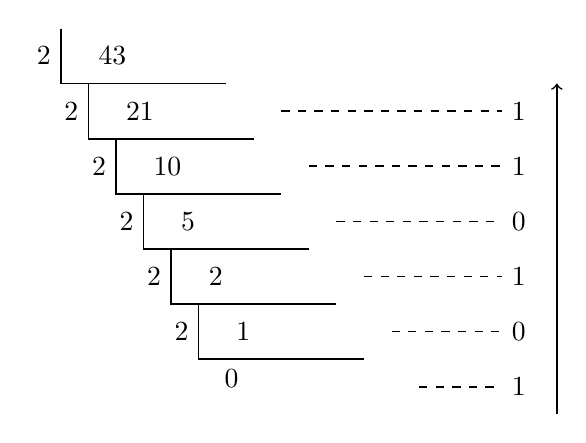
\begin{tikzpicture}[semithick,scale=0.7]
                    \draw (0,0) |- (3,-1) node [left,pos=0.25] {2} node [right,pos=0.25] {\quad 43};
                    \foreach \s [count=\i] in{21,10,5,2}
                    \draw [shift={({0.5*\i},-\i)}] (0,0) |- (3,-1) node [left,pos=0.25] {2} node [right,pos=0.25] {\quad \s};
                    \draw [shift={({2.5},-5)}] (0,0) |- (3,-1) node [left,pos=0.25] {2} node [right,pos=0.25] {\quad 1} node [below,pos=0.6] {0};
                    \foreach \s [count=\i] in{1,1,0,1,0,1}
                    \draw [dashed,shift={(0,1-\i)}] ({3.5+0.5*\i},-1.5) -- (8,-1.5) node [right] {\s};
                    \draw [->] (9,-7) -- (9,-1);
                \end{tikzpicture}            
        \end{center}
        \qquad \quad 43 D $=101011$ B
        }
        \only<2>{
            \begin{center}
                \only<2>{
                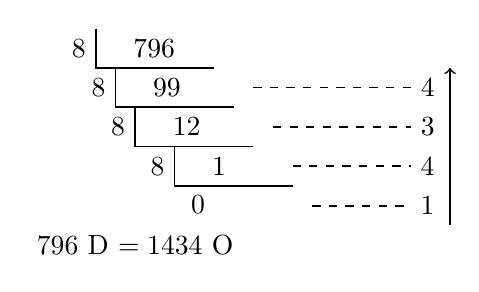
\begin{tikzpicture}[semithick,scale=0.5]
                    \draw (0,0) |- (3,-1) node [left,pos=0.25] {8} node [right,pos=0.25] {\quad 796};
                    \foreach \s [count=\i] in{99,12}
                        \draw [shift={({0.5*\i},-\i)}] (0,0) |- (3,-1) node [left,pos=0.25] {8} node [right,pos=0.25] {\quad \s};
                    \draw [shift={({2},-3)}] (0,0) |- (3,-1) node [left,pos=0.25] {8} node [right,pos=0.25] {\quad 1} node [below,pos=0.6] {0};
                    \foreach \s [count=\i] in{4,3,4,1}
                    \draw [dashed,shift={(0,1-\i)}] ({3.5+0.5*\i},-1.5) -- (8,-1.5) node [right] {\s};
                    \draw [->] (9,-5) -- (9,-1);
                    \node at (1,-5.5) {796 D $=1434$ O};
                \end{tikzpicture}

                \medskip
                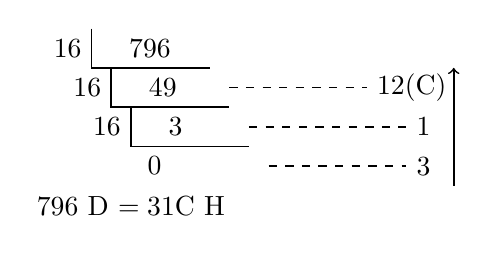
\begin{tikzpicture}[semithick,scale=0.5]
                    \draw (0,0) |- (3,-1) node [left,pos=0.25] {16} node [right,pos=0.25] {\quad 796};
                    \draw [shift={({0.5},-1)}] (0,0) |- (3,-1) node [left,pos=0.25] {16} node [right,pos=0.25] {\quad 49};
                    \draw [shift={({1},-2)}] (0,0) |- (3,-1) node [left,pos=0.25] {16} node [right,pos=0.25] {\quad 3} node [below,pos=0.6] {0};
                    \draw [dashed] (3.5,-1.5) -- (7,-1.5) node [right] {12(C)};
                    \foreach \s [count=\i] in{1,3}
                    \draw [dashed,shift={(0,-\i)}] ({3.5+0.5*\i},-1.5) -- (8,-1.5) node [right] {\s};
                    \draw [->] (9.2,-4) -- (9.2,-1);
                    \node at (1,-4.5) {796 D $=31$C\ H};
                \end{tikzpicture}
            }
            \end{center}
        }
    \end{minipage}
\end{frame}


\begin{frame}[t]
    \frametitle{}
    \begin{question}
        \begin{enumerate}
          \item 二进制转十进制
          
          \begin{itemize}
            \item 11001100
            \item 11111111 (8个1)
          \end{itemize}
          \item 十进制转二进制
          
          \begin{itemize}
            \item 1234.5
            \item 1024
          \end{itemize}
        \end{enumerate}
    \end{question}
\end{frame}



\begin{frame}
    \frametitle{十进制 → 二、八、十六进制}
        \begin{minipage}{0.4\linewidth}
            \begin{center}
                \begin{tikzpicture}[thick,node distance=2cm,scale=1,every node/.style={scale=1}]
                    \node (10) [draw,circle] {十进制};
                    \node (8) [draw,rectangle,above of=10,xshift=-2cm] {八进制};
                    \node (16) [draw,rectangle,above of=10,xshift=2cm] {十六进制};
                    \node (2) [draw,rectangle,below of=10] {二进制};
                    \draw [->,MediumPurple1] (10.north west) to [bend right=30] (8.south east);
                    \draw [->,MediumPurple1] (10.north east) to [bend right=30] (16.south west);
                    \draw [->,MediumPurple1] (10.south) to [bend right=30] (2.north);
                \end{tikzpicture}
            \end{center}
    \end{minipage}\hfill
    \begin{minipage}{0.58\linewidth}        
        \highlight{小数部分} 乘2/8/16取整，顺序排列。
        \only<1>{
            \begin{enumerate}
                \item 0.625 D $=0.101$ B
                    \begin{align*}
                    0.625 \times 2 & = 1.25 \\
                    0.25 \times 2 & = 0.5 \\
                    0.5  \times 2 & = 1 
                    \end{align*}
                \item 0.625 D $=0.5$ O         
                \[0.625 \times 8  = 5\]
                \item 0.625 D $=0.\mathrm{A\ H}$          
                \[0.625 \times 16  = 10\]
              \end{enumerate}
        } 
        \only<2>{
            \begin{itemize}
              \item[4.] 0.1 D$=0.0001100110011\cdots\mathrm{B}$
                \begin{align*}
                    0.1 \times 2 & = 0.2 \\
                    0.2 \times 2 & = 0.4 \\
                    0.4 \times 2 & = 0.8 \\
                    0.8 \times 2 & = 1.6 \\
                    0.6 \times 2 & = 1.2 \\
                    0.2 \times 2 & = 0.4 \\
                    0.4 \times 2 & = 0.8 \\
                    0.8 \times 2 & = 1.6 \\
                    \cdots \cdots 
                \end{align*}
            \end{itemize}
        }
    \end{minipage}
\end{frame}


\begin{frame}
    \frametitle{二进制 ↔ 八、十六进制}
    \begin{minipage}{0.4\linewidth}
        \begin{center}
            \begin{tikzpicture}[thick,node distance=2cm,scale=1,every node/.style={scale=1}]
                \node (10) [circle] {};
                \node (8) [draw,rectangle,above of=10,xshift=-2cm] {八进制};
                \node (16) [draw,rectangle,above of=10,xshift=2cm] {十六进制};
                \node (2) [draw,rectangle,below of=10] {二进制};
                \draw [->,Chartreuse3] (2.north west) -- (8);
                \draw [->,Chartreuse3] (2.north east) -- (16);
                \draw [->,Chartreuse3] (8) to [bend right=45] (2);
                \draw [->,Chartreuse3] (16) to [bend left=45] (2);
            \end{tikzpicture}
        \end{center}
    \end{minipage}\hfill
    \begin{minipage}{0.58\linewidth}
        \only<1>{
            \begin{itemize}
                \item 二进制 → 八进制：三合一
                
                \begin{center}
                  \begin{tikzpicture}[semithick]
                      \node at (0,0) {11010111.0100111};
                      \draw [->] (0,-0.2) -- (0,-0.8);
                      \node at (0,-1) {\culine{\red{0}11} \culine{010} \culine{111}.\culine{010} \culine{011} \culine{1\red{00}}};
                      \draw [->] (-0.05,-1.3) -- (-2,-1.3) node [below,midway] {\tiny 画线};
                      \draw [->] (0.05,-1.3) -- (2,-1.3) node [below,midway] {\tiny 画线};
                      \draw [->] (-1.65,-1.7) -- (-1.65,-2.2) node [below] {3};
                      \foreach \x [count=\i] in {2,7,2,3,4}
                          \draw [->,shift={({0.67*\i,0})}] (-1.65,-1.7) -- (-1.65,-2.2) node [below] {\x};
                      \node at (0,-2.6) {.};
                  \end{tikzpicture}
              \end{center}
                \item 二进制 → 十六进制：四合一
                
                \begin{center}
                  \begin{tikzpicture}[semithick]
                      \node at (0,0) {11010111.0100111};
                      \draw [->] (0,-0.2) -- (0,-0.8);
                      \node at (0,-1) {\culine{1101} \culine{0111}.\culine{0100} \culine{111\red{0}}};
                      \draw [->] (-0.05,-1.3) -- (-1.7,-1.3) node [below,midway] {\tiny 画线};
                      \draw [->] (0.05,-1.3) -- (1.7,-1.3) node [below,midway] {\tiny 画线};
                      \draw [->] (-1.25,-1.7) -- (-1.25,-2.2) node [below] {D};
                      \foreach \x [count=\i] in {7,4,E}
                          \draw [->,shift={({0.85*\i,0})}] (-1.25,-1.7) -- (-1.25,-2.2) node [below] {\x};
                      \node at (0,-2.6) {.};
                  \end{tikzpicture}
                \end{center}
              \end{itemize}
        }
        \only<2>{
            \begin{itemize}
              \item 八进制 → 二进制：一分三
              
              \begin{center}
                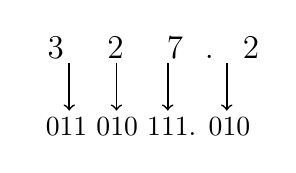
\begin{tikzpicture}[semithick]
                    \node at (0,0) {\large \culine{ 3 }\ \ \culine{ 2 }\ \ \culine{ 7 } . \culine{ 2 }};
                    \node at (0,-1) {011 010 111. 010};
                    \foreach \x in {-1,-0.4,0.25,1}
                        \draw [->] (\x,-0.2) -- (\x,-0.8);
                \end{tikzpicture}
              \end{center}
              \item 十六进制 → 二进制：一分四
              
              \begin{center}
                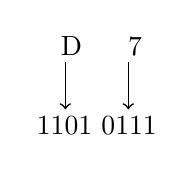
\begin{tikzpicture}[semithick]
                    \node at (0,0) {\cyan{\culine{ \black{D} }}\quad \culine{ 7 }};
                    \node at (0,-1) {1101 0111};
                    \foreach \x in {-0.4,0.4}
                        \draw [->] (\x,-0.2) -- (\x,-0.8);
                \end{tikzpicture}
              \end{center}
            \end{itemize}
        }
    \end{minipage}
\end{frame}


\begin{frame}
    \frametitle{进制转换速查表}
    \begin{minipage}{0.48\linewidth}
        \begin{table}
            \centering
            \begin{tabular}{cccc}
                \toprule
                十进制 & 二进制 & 八进制 & 十六进制 \\ \midrule 
                0 & 0 & 0 & 0 \\
                1 & 1 & 1 & 1 \\
                2 & 10 & 2 & 2 \\
                3 & 11 & 3 & 3 \\
                4 & 100 & 4 & 4 \\
                5 & 101 & 5 & 5 \\
                6 & 110 & 6 & 6 \\
                7 & 111 & 7 & 7 \\ \bottomrule            
            \end{tabular}
        \end{table}
    \end{minipage}\hfill
    \begin{minipage}{0.48\linewidth}
        \begin{table}
            \centering
            \begin{tabular}{cccc}
                \toprule
                十进制 & 二进制 & 八进制 & 十六进制 \\ \midrule 
                8 & 1000 & 10 & 8 \\
                9 & 1001 & 11 & 9 \\
                10 & 1010 & 12 & A \\
                11 & 1011 & 13 & B \\
                12 & 1100 & 14 & C \\
                13 & 1101 & 15 & D \\
                14 & 1110 & 16 & E \\
                15 & 1111 & 17 & F \\ \bottomrule            
            \end{tabular}
        \end{table}
    \end{minipage}
\end{frame}


\begin{frame}
    \frametitle{八进制 ↔ 十六进制}
    \begin{minipage}{0.4\linewidth}
        \begin{center}
            \begin{tikzpicture}[thick,node distance=4cm,scale=1,every node/.style={scale=1}]
                \node (8) [draw,rectangle] {八进制};
                \node (16) [draw,rectangle,right of=8] {十六进制};
                \draw [->,cyan,dashed] (8.north) to [bend left=60] node [midway,circle,draw,red] {2} (16.north) ;
                \draw [->,cyan,dashed] (16.south) to [bend left=60] node [midway,circle,draw,red] {2}  (8.south);
            \end{tikzpicture}
        \end{center}
    \end{minipage}\hfill
    \begin{minipage}{0.58\linewidth}
        方法：先转换为二进制，再转换为八(十六)进制
        \begin{center}
            \begin{tikzpicture}[semithick,scale=2]
                \node at (0,-0.4) {.};
                \foreach \x [count=\i] in {2,7,2,3,4}
                    \draw [->,shift={({0.67*\i,0})}] (-1.65,-0.5) node [above] {\x} -- (-1.65,-1);
                \node at (0,-1.2) {\red{0}\ \ 1\ \ 1\quad \ 0\ \ 1\ \ 0\quad \ 1\ \ 1\ \ 1\ . 0\ \ 1\ \ 0\quad \ 0\ \ 1\ \ 1\quad \ 1\ \ \red{0\ \ 0}};
                \draw [cyan] (-0.1,-1.4) -- (-0.9,-1.4);
                \draw [cyan] (-1.0,-1.4) -- (-1.8,-1.4);
                \draw [cyan] (0.1,-1.4) -- (0.9,-1.4);
                \draw [cyan] (1.0,-1.4) -- (1.8,-1.4);
                \draw [->] (-0.05,-1.5) -- (-2,-1.5) node [below,midway] {\tiny 画线};
                \draw [->] (0.05,-1.5) -- (2,-1.5) node [below,midway] {\tiny 画线};
                \draw [->] (-1.65,-0.5) node [above] {3} -- (-1.65,-1) ;
                \foreach \x [count=\i] in {D,7,4,E}
                    \draw [->,shift={({0.9*\i,0})}] (-2.25,-1.9) -- (-2.25,-2) node [below] {\x};
                \node at (0,-2.3) {.};
            \end{tikzpicture}
        \end{center}
    \end{minipage}
\end{frame}

\begin{frame}[t]
    \frametitle{}
    \begin{question}
        十六进制转八进制
          \begin{itemize}
            \item ABC
            \item 123
          \end{itemize}
    \end{question}
\end{frame}


\subsection{数在计算机中的二进制表示}


\begin{frame}[t]
    \frametitle{数的二进制表示}
    \begin{question}
        \begin{enumerate}
            \item 小数怎么表示？
            \item 负数怎么表示？
            \item 用多少bit表示？
            \item 加减法怎么运算？
          \end{enumerate}
    \end{question}
\end{frame}


\begin{frame}
    \frametitle{数的位数与表示范围}
    一个字节可以表示的整数的范围是？
      \begin{center}
        \hspace{2.5em}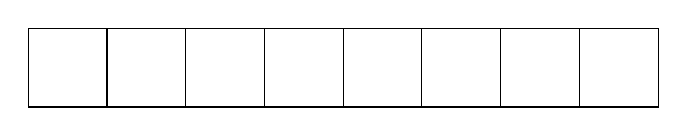
\begin{tikzpicture}
            \foreach \x in {0,1,2,3,4,5,6,7}
            \draw [shift={({\x},0)}] (0,0) rectangle (1,1);
        \end{tikzpicture}
      \end{center}
      \vspace{-1em}
      \pause
    \begin{itemize}
      \item 无符号整数：$(00000000)_2 \sim (11111111)_2$ 即 $0\sim255$
      \item 有符号整数
      
      用最高位表示符号位（0正1负），剩余七位用来表示数据位\footnote{这种方法有一个缺陷，就是会有$+0$和$-0$两个$0$，能够表示的数据只有$-127 \sim  +127$，同时使用两个位组合表示同一个数字有些浪费，\highlight{补码}很好的解决了这一问题。}。
        \begin{center}
            \begin{tikzpicture}
                \draw [fill=Pink2] (0,0) rectangle (1,1) node {};
                \foreach \x in {1,2,3,4,5,6,7}
                \draw [shift={(\x,0)},fill=PaleGreen2] (0,0) rectangle (1,1);
                \draw [<-] (0.5,0) -- (0.5,-0.5) node [below] {符号位};
                \draw [decorate,decoration={brace,mirror,amplitude=0.4cm,raise= 0.1cm}] (1,0) -- (8,0) node [below,midway,shift={(0,-0.5)}] {数据位};
            \end{tikzpicture}
        \end{center}
    \end{itemize}
\end{frame}


\begin{frame}
    \frametitle{整数}
    无符号整数没有符号位，全部表示真值；有符号整数，最高位作为符号位，其他表示真值。
    \begin{multicols}{2}
        \begin{itemize}
          \item 有符号整数\footnote{signed，有符号，通常省略}
            \begin{itemize}
              \item short \hspace{2.5em} 2字节
              \item int \hspace{3.4em} 4字节
              \item long \hspace{2.75em} 4字节\footnote{不同的环境下有不同的长度}
              \item long long \quad 8字节
            \end{itemize}
          \item 无符号整数
          \begin{itemize}
            \item unsigned short \hspace{2.5em} 2字节
            \item unsigned int \hspace{3.4em} 4字节
            \item unsigned long \hspace{2.75em} 4字节
            \item unsigned long long \quad 8字节
          \end{itemize}
        \end{itemize}
    \end{multicols}
\end{frame}


\begin{frame}[t]
    \frametitle{}
    \begin{example}
        写出8位二进制数-100110 B在计算机中的表示。
    \end{example}
    \pause
    \begin{center}
        \begin{tikzpicture}
            \draw [fill=Pink2] (0,0) rectangle (1,1) node [midway] {1};
            \foreach \x/\y in {1/0,2/1,3/0,4/0,5/1,6/1,7/0}
            \draw [shift={(\x,0)},fill=PaleGreen2] (0,0) rectangle (1,1) node [midway] {\y};
            \draw [<-] (0.5,0) -- (0.5,-0.5) node [below] {符号位};
            \draw [decorate,decoration={brace,mirror,amplitude=0.4cm,raise= 0.1cm}] (1,0) -- (8,0) node [below,midway,shift={(0,-0.5)}] {数据位};
        \end{tikzpicture}
    \end{center}
\end{frame}

\begin{frame}
    \frametitle{二进制加法}
    二进制加法是逢二进一
    \Huge{\begin{align*}
        1001 \\
        \underline{+\quad 1101} \\
        =\ 10110
    \end{align*}}
\end{frame}

\begin{frame}[t]
    \frametitle{}
    \begin{question}
        计算机只会做加法，那么计算机如何计算$1-1=?$
        \[2-1=2+(-1) \]
    \end{question}
    \begin{align*}
        00000010 \\
        \underline{+\ \ 10000001} \\
        =\ 10000011
    \end{align*}
    \[\red{2 - 1 = -3?}\]
    让计算机辨别“符号位”会让计算机的基础电路设计变得十分复杂，能不能设计一种方法，让符号位直接参与运算，且能得到正确的结果？
\end{frame}


\begin{frame}
    \frametitle{原码、反码}
    \notice 既然一个负数是一个正数的相反数，那干脆用一个正数按位取反来表示负数试试。

    \begin{table}[]
        \begin{tabular}{@{}cccc>{\columncolor{maincolor!20}}cc@{}}
            \bottomrule
        正数  & 原码/反码 & 负数  & 原码 & 反码  \\ \hline
        0 & 00000000 & -0  & 10000000 & 11111111  \\
        1 & 00000001 & -1  & 10000001 & 11111110  \\
        2 & 00000010 & -2  & 10000010 & 11111101  \\
        $\vdots$  & $\vdots$   & $\vdots$  & $\vdots$    & $\vdots$  \\
        125 & 01111101 & -125  & 11111101 & 10000010 \\
        126 & 01111110 & -126 & 11111110 & 10000001 \\
        127 & 01111111 & -127 & 11111111 & 10000000 \\ \toprule
        \end{tabular}
        \end{table}
        
    \highlight{反码}正数的反码是其本身。负数的反码是在其原码的基础上，符号位不变，其余各位取反。
\end{frame}

\begin{frame}
    \frametitle{原码、反码}
    \begin{question}
        \begin{align*}
            2 - 1 = 2 + (-1) =? \\
            0000 0010 \ \text{[反]}&\\
            \underline{+\ \ \ 1111 1110 \ \text{[反]}}&  \\
            =100000000 \ \text{[反]}& \text{\quad --- 最高位产生进位，舍弃最高位，结果+1} \\
            =\ \ 00000001 \ \text{[反]}& \\
            =\ \ 00000001 \ \text{[原]}&
        \end{align*}
    \end{question}

    反码解决了原码做减法的问题，但是还有一个问题没有解决：

    $[+0] \ [-0]$同时存在打破了系统编码的连续性和一致性，应该极力规避。
\end{frame}

\begin{frame}
    \frametitle{时钟计数法}
    \begin{minipage}{0.48\linewidth}
        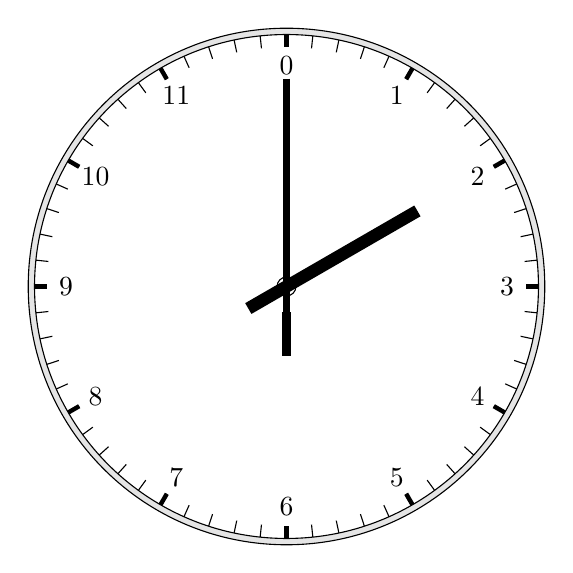
\begin{tikzpicture}[scale=0.8]
            \filldraw[fill=gray!20](0,0)circle(4.1cm);
            \filldraw[fill=white](0,0)circle(4cm);
            \foreach \x in {6,12,...,360}
            \draw(\x:4)--(\x:3.8);
            \foreach \x in {0,30,...,330}
            \draw[ultra thick](\x:4)--(\x:3.8);
            \foreach \y/\z in {0/3,30/2,60/1,90/0,120/11,150/10,180/9,210/8,240/7,270/6,300/5,-30/4}
            \node at (\y:3.5){\z};
            \draw (0,0)circle(0.15);
            \draw[line width=4.5pt,rotate=-60](90:2.4)--(-90:0.7);
            \draw[line width=2.5pt,rotate=-180](-90:3.3)--(90:0.65);
            \draw[line width=3.5pt,rotate=0](-90:1.1)--(-90:0.4);
            \end{tikzpicture}
    \end{minipage}\hfill
    \begin{minipage}{0.48\linewidth}
        \only<1>{
            \Huge{\begin{align*}
                2 - 1 &= 1 \\
                2 + ? &= 1
            \end{align*}} 
        }
        \only<2>{
            \Huge{\begin{align*}
                2 - 1 &= 1 \\
                2 + 11 &= 1
            \end{align*}} 
        }
        \pause
        \Huge{\begin{align*}
            2 - 1 =2 + 11
        \end{align*}} 
        
    \end{minipage}
\end{frame}

\begin{frame}
    \frametitle{补码}
    \only<1>{        
        \begin{center}
            \begin{tikzpicture}[thick]
                % \draw [fill=Pink1,dashed] (0,0) rectangle (1,1) node [midway] {1};
                \foreach \x/\y in {1/0,2/0,3/0,4/0,5/0,6/0,7/0,8/1}
                \draw [shift={(\x,0)},fill=PaleGreen2] (0,0) rectangle (1,1) node [midway] {\y};
                \node at (9.7,0) {};
                \foreach \x/\y in {1/?,2/?,3/?,4/?,5/?,6/?,7/?,8/?}
                \draw [shift={(\x,1.5)}] (0,0) rectangle (1,1) node [midway] {\y};
                \foreach \x/\y in {1/0,2/0,3/0,4/0,5/0,6/0,7/1,8/0}
                \draw [shift={(\x,3)},fill=PaleGreen2] (0,0) rectangle (1,1) node [midway] {\y};
                \draw (-1,1.25) -- (9,1.25);
                \node at (-0.5,0.5) {$=$};
                \node at (-0.5,2) {$+$};
                \node at (10,0.5) {1};
                \node [rotate=90] at (10,1.25) {$=$};
                \node at (10,2) {(-1)};
                \node at (10,2.75) {$+$};
                \node at (10,3.5) {2};
                \node at (-1.5,-1) {};
            \end{tikzpicture}
        \end{center}
    }
    \only<2>{
        \begin{center}
            \begin{tikzpicture}[thick]
                \draw [fill=Pink1,dashed] (0,0) rectangle (1,1) node [midway] {1};
                \foreach \x/\y in {1/0,2/0,3/0,4/0,5/0,6/0,7/0,8/1}
                \draw [shift={(\x,0)},fill=PaleGreen2] (0,0) rectangle (1,1) node [midway] {\y};
                \draw [<-] (0.5,0) -- (0.5,-0.5) node [below] {最高位进位，溢出舍弃};
                \node at (9.7,0) {};
                \foreach \x/\y in {1/?,2/?,3/?,4/?,5/?,6/?,7/?,8/?}
                \draw [shift={(\x,1.5)}] (0,0) rectangle (1,1) node [midway] {\y};
                \foreach \x/\y in {1/0,2/0,3/0,4/0,5/0,6/0,7/1,8/0}
                \draw [shift={(\x,3)},fill=PaleGreen2] (0,0) rectangle (1,1) node [midway] {\y};
                \draw (-1,1.25) -- (9,1.25);
                \node at (-0.5,0.5) {$=$};
                \node at (-0.5,2) {$+$};
                \node at (10,0.5) {1};
                \node [rotate=90] at (10,1.25) {$=$};
                \node at (10,2) {(?)};
                \node at (10,2.75) {$+$};
                \node at (10,3.5) {2};
            \end{tikzpicture}
        \end{center}
    }
    \only<3>{
        \begin{center}
            \begin{tikzpicture}[thick]
                \draw [fill=Pink1,dashed] (0,0) rectangle (1,1) node [midway] {1};
                \foreach \x/\y in {1/0,2/0,3/0,4/0,5/0,6/0,7/0,8/1}
                \draw [shift={(\x,0)},fill=PaleGreen2] (0,0) rectangle (1,1) node [midway] {\y};
                \draw [<-] (0.5,0) -- (0.5,-0.5) node [below] {最高位进位，溢出舍弃};
                \node at (9.7,0) {};
                \foreach \x/\y in {1/1,2/1,3/1,4/1,5/1,6/1,7/1,8/1}
                \draw [shift={(\x,1.5)}] (0,0) rectangle (1,1) node [midway] {\y};
                \foreach \x/\y in {1/0,2/0,3/0,4/0,5/0,6/0,7/1,8/0}
                \draw [shift={(\x,3)},fill=PaleGreen2] (0,0) rectangle (1,1) node [midway] {\y};
                \draw (-1,1.25) -- (9,1.25);
                \node at (-0.5,0.5) {$=$};
                \node at (-0.5,2) {$+$};
                \node at (10,0.5) {1};
                \node [rotate=90] at (10,1.25) {$=$};
                \node at (10,2) {255};
                \node at (10,2.75) {$+$};
                \node at (10,3.5) {2};
            \end{tikzpicture}
        \end{center}
    }
    \onslide<3>{
        \highlight{补码}\quad $-x = 2^n - x$，n为位数。
    }
    
\end{frame}

\begin{frame}
    \frametitle{原码、反码、补码}
    在计算机中通常以二进制补码的形式存储整数。
% \begin{table}[]
%     \begin{tabular}{@{}cccccccc@{}}
%     \toprule
%              & 原码  & 反码  & 补码  &          & 原码   & 反码   & 补码   \\ \midrule
%     00000000 & 0   & 0   & 0   & 10000000 & -0   & -127   & -128 \\
%     00000001 & 1   & 1   & 1   & 10000001 & -1   & -126 & -127 \\
%     00000010 & 2   & 2   & 2   & 10000010 & -2   & -125 & -126 \\
%     $\vdots$  & $\vdots$   & $\vdots$  & $\vdots$    & $\vdots$    & $\vdots$    & $\vdots$    & $\vdots$    \\
%     01111101 & 125 & 125 & 125 & 11111101 & -125 & -2   & -3   \\
%     01111110 & 126 & 126 & 126 & 11111110 & -126 & -1   & -2   \\
%     01111111 & 127 & 127 & 127 & 11111111 & -127 & -0   & -1   \\ \bottomrule
%     \end{tabular}
%     \end{table}
\begin{table}[]
    \begin{tabular}{@{}ccccc>{\columncolor{maincolor!20}}cc@{}}
        \bottomrule
    正数  & 原码/反码/补码 & 负数  & 原码 & 反码 & 补码 \\ \hline
    0 & 00000000 & -0  & 10000000 & 11111111 & - \\
    1 & 00000001 & -1  & 10000001 & 11111110 & 11111111 \\
    2 & 00000010 & -2  & 10000010 & 11111101 & 11111110 \\
    $\vdots$  & $\vdots$   & $\vdots$  & $\vdots$    & $\vdots$ & $\vdots$ \\
    125 & 01111101 & -125  & 11111101 & 10000010 & 10000011 \\
    126 & 01111110 & -126 & 11111110 & 10000001 & 10000010 \\
    127 & 01111111 & -127 & 11111111 & 10000000 & 10000001 \\ 
    - & - & -128 & - & - & 10000000 \\ \toprule
    \end{tabular}
    \end{table}
\end{frame}


\begin{frame}
    \frametitle{定点数}
    小数点如何表示？约定计算机中小数点的位置。

    \begin{enumerate}
      \item 纯整数：小数点约定在最低位的右边 (100 D $=$ 1100100 B)
      \begin{center}
        \begin{tikzpicture}
            \draw [fill=Pink2] (0,0) rectangle (1,1) node [midway] {0};
            \foreach \x/\y in {1/1,2/1,3/0,4/0,5/1,6/0,7/0}
            \draw [shift={(\x,0)},fill=PaleGreen2] (0,0) rectangle (1,1) node [midway] {\y};
            \draw [<-] (0.5,0) -- (0.5,-0.5) node [below] {符号位};
            \draw [decorate,decoration={brace,mirror,amplitude=0.4cm,raise= 0.1cm}] (1.2,0) -- (7.8,0) node [below,midway,shift={(0,-0.5)}] {数据位};
            \draw [<-] (8,0) -- (8,-0.5) node [below] {小数点};
        \end{tikzpicture}
    \end{center}
      \item 纯小数：小数点约定在符号位之后 ($-$0.125 D $=$ $-$0.001 B)
      \begin{center}
        \begin{tikzpicture}
            \draw [fill=Pink2] (0,0) rectangle (1,1) node [midway] {1};
            \foreach \x/\y in {1/0,2/0,3/1,4/0,5/0,6/0,7/0}
            \draw [shift={(\x,0)},fill=PaleGreen2] (0,0) rectangle (1,1) node [midway] {\y};
            \draw [<-] (0.5,0) -- (-0.5,-0.5) node [below] {符号位};
            \draw [decorate,decoration={brace,mirror,amplitude=0.4cm,raise= 0.1cm}] (1.2,0) -- (7.8,0) node [below,midway,shift={(0,-0.5)}] {数据位};
            \draw [<-] (1,0) -- (1,-0.5) node [below] {小数点};
            \node at (9.7,0) {};
        \end{tikzpicture}
    \end{center}
    \end{enumerate}
\end{frame}

\begin{frame}[t]
    \frametitle{定点数}
    \begin{itemize}
      \item[3.] 整数+小数 (6.125 D $=$ 110.001 B)
    \end{itemize}
      \begin{center}
        \begin{tikzpicture}
            \foreach \x/\y/\c in {0/0/Pink2,1/0/PaleGreen2,2/1/PaleGreen2,3/1/PaleGreen2,4/0/PaleGreen2,5/0/PaleTurquoise2,6/0/PaleTurquoise2,7/1/PaleTurquoise2}
            \draw [shift={(\x,0)},fill=\c] (0,0) rectangle (1,1) node [midway] {\y};
            \draw [<-] (0.5,0) -- (0.5,-0.5) node [below] {符号位};
            \draw [decorate,decoration={brace,mirror,amplitude=0.4cm,raise= 0.1cm}] (1.2,0) -- (4.8,0) node [below,midway,shift={(0,-0.5)}] {整数位};  
            \draw [decorate,decoration={brace,mirror,amplitude=0.4cm,raise= 0.1cm}] (5.2,0) -- (7.8,0) node [below,midway,shift={(0,-0.5)}] {小数位};           
            \draw [<-] (5,0) -- (5,-0.5) node [below] {小数点};
            \node at (9.7,0) {};
        \end{tikzpicture}
    \end{center}
    \pause
    \only<2>{
    \begin{question}
        我们约定了用 4 位表示整数部分，后 3 位表示小数部分，此时这个整数部分的二进制最大值只能是 1111，即十进制的 15，小数部分的二进制最大只能表示 0.111，即十进制的 0.875。如果我们想要表示更大范围的值，怎么办？
        \vspace{-1em}
            \begin{multicols}{2}
                \begin{itemize}
                    \item[] 
                  \end{itemize}
            \end{multicols}
    \end{question}
    }
    \only<3>{
    \begin{question}
        我们约定了用 4 位表示整数部分，后 3 位表示小数部分，此时这个整数部分的二进制最大值只能是 1111，即十进制的 15，小数部分的二进制最大只能表示 0.111，即十进制的 0.875。如果我们想要表示更大范围的值，怎么办？
        \vspace{-1em}
            \begin{multicols}{2}
                \begin{itemize}
                    \item 扩大 bit 的宽度
                    \item 改变小数点的位置
                  \end{itemize}
            \end{multicols}
    \end{question}
    }
\end{frame}

\begin{frame}
    \frametitle{定点数}
    \begin{center}
        \begin{tikzpicture}[scale=0.85]
            \draw [fill=Pink2] (0,0) rectangle (1,1) node {};
            \foreach \x in {1,2,3,4,5,6,7,8,9}
            \draw [shift={(\x,0)},fill=PaleGreen2] (0,0) rectangle (1,1);
            \foreach \x in {1,2,3,4,5,6}
            \draw [shift={({9+\x},0)},fill=PaleTurquoise2] (0,0) rectangle (1,1);
            \draw [<-] (0.5,0) -- (0.5,-0.5) node [below] {符号位};
            \draw [decorate,decoration={brace,mirror,amplitude=0.4cm,raise= 0.1cm}] (1.2,0) -- (9.8,0) node [below,midway,shift={(0,-0.5)}] {整数位};
            \draw [decorate,decoration={brace,mirror,amplitude=0.4cm,raise= 0.1cm}] (10.2,0) -- (15.8,0) node [below,midway,shift={(0,-0.5)}] {小数位};
            \draw [<-] (10,0) -- (10,-0.5) node [below] {小数点};
        \end{tikzpicture}

        \begin{tikzpicture}[scale=0.85]
            \draw [fill=Pink2] (0,0) rectangle (1,1) node {};
            \foreach \x in {1,2,3,4,5,6,7}
            \draw [shift={(\x,0)},fill=PaleGreen2] (0,0) rectangle (1,1);
            \foreach \x in {1,2,3,4,5,6,7,8}
            \draw [shift={({7+\x},0)},fill=PaleTurquoise2] (0,0) rectangle (1,1);
            \draw [<-] (0.5,0) -- (0.5,-0.5) node [below] {符号位};
            \draw [decorate,decoration={brace,mirror,amplitude=0.4cm,raise= 0.1cm}] (1.2,0) -- (7.8,0) node [below,midway,shift={(0,-0.5)}] {整数位};
            \draw [decorate,decoration={brace,mirror,amplitude=0.4cm,raise= 0.1cm}] (8.2,0) -- (15.8,0) node [below,midway,shift={(0,-0.5)}] {小数位};
            \draw [<-] (8,0) -- (8,-0.5) node [below] {小数点};
        \end{tikzpicture}
    \end{center}
    \pause
    \notice 不管如何约定小数点的位置，都会存在以下问题:
    \begin{itemize}
      \item 数值的表示范围有限（小数点越靠左，整个数值范围越小）
      \item 数值的精度范围有限（小数点越靠右，数值精度越低）
    \end{itemize}
\end{frame}

\begin{frame}[t]
    \frametitle{}
    \begin{question}
        当我们表示非常大或非常小的数字时是如何表示的？
    \end{question}

    \bigskip
    \begin{minipage}{0.28\linewidth}
    \begin{itemize}
        \item 光速
        \item 世界总人口(80亿)
        \item 阿伏伽德罗常数
        \item 普朗克常量
        \item 电子电荷量
      \end{itemize}
    \end{minipage}\hfill \pause
    \begin{minipage}{0.68\linewidth}
    \begin{itemize}
        \item $c= \SI{3e8}{m.s^{-1}}$
        \item $8.0 \times 10^9$
        \item $N_\mathrm{A} = \SI{6.02e23}{mol^{-1}}$
        \item $h=\SI{6.62607015e-34}{J.s}$
        \item $e=\SI{1.602e-19}{C}$
      \end{itemize}
    \end{minipage}

    \bigskip
    \qquad 当我们要标记或运算某个较大或较小且位数较多的数时，用\highlight{科学记数法}免去浪费很多空间和时间。
\end{frame}


\begin{frame}
    \frametitle{浮点数}
    \highlight{浮点数}是采用科学记数法的方式来表示的。

    十进制小数 8.345，用科学记数法表示，可以有多种方式：
    \begin{align*}
    8.345 &= 8.345 \times 10^0 \\
    8.345 &= 83.45 \times 10^{-1} \\
    8.345 &= 834.5 \times 10^{-2}
    \end{align*}
    用这种科学记数法的方式表示小数时，小数点的位置就变得「漂浮不定」了，这就是相对于定点数，浮点数名字的由来。

    使用同样的规则，对于二进制数，我们也可以用科学记数法表示，把基数 10 换成 2 即可。
\end{frame}

\begin{frame}
    \frametitle{浮点数}    
    浮点数的格式可以写成这样：$\mathrm{N} = (-1)^\mathrm{S} \times \mathrm{M} \times \mathrm{R}^\mathrm{E}$
    \begin{itemize}
        \item S：符号位，取值 0 或 1，决定一个数字的符号，0 表示正，1 表示负
        \item M：尾数，用小数表示
        \item R：基数，表示十进制数 R 就是 10，表示二进制数 R 就是 2
        \item E：指数，用整数表示
      \end{itemize}
      如果我们要在计算机中，用浮点数表示一个数字，只需要确认这几个变量即可。
      \begin{center}
        \begin{tikzpicture}[scale=0.85]
            \draw [fill=Pink2] (0,0) rectangle (1,1) node {};
            \foreach \x in {1,2,3,4,5,6,7,8}
            \draw [shift={(\x,0)},fill=PaleGreen2] (0,0) rectangle (1,1);
            \foreach \x in {1,2,3,4,5,6,7}
            \draw [shift={({8+\x},0)},fill=PaleTurquoise2] (0,0) rectangle (1,1);
            \draw [<-] (0.5,0) -- (0.5,-0.5) node [below] {符号位};
            \draw [decorate,decoration={brace,mirror,amplitude=0.4cm,raise= 0.1cm}] (1.2,0) -- (8.8,0) node [below,midway,shift={(0,-0.5)}] {指数E};
            \draw [decorate,decoration={brace,mirror,amplitude=0.4cm,raise= 0.1cm}] (9.2,0) -- (15.8,0) node [below,midway,shift={(0,-0.5)}] {尾数M};
        \end{tikzpicture}
      \end{center}
\end{frame}


\begin{frame}[t]
    \frametitle{}
    \begin{example}
        将80亿用二进制科学记数法表示
        \begin{align*}
            8 \times 10^9 \mathrm{\ D}&= 111011100110101100101000000000000  \mathrm{\ B} \\
            &= 1.110111\cdots \times 2^{32} \\
            32 \mathrm{\ D}&=100000 \mathrm{\ B}
        \end{align*}
    \end{example}
    \only<1>{
        \begin{center}
            \begin{tikzpicture}[scale=0.85]
                \draw [fill=Pink2] (0,0) rectangle (1,1) node {};
                \foreach \x in {1,2,3,4,5,6,7,8}
                \draw [shift={(\x,0)},fill=PaleGreen2] (0,0) rectangle (1,1);
                \foreach \x in {1,2,3,4,5,6,7}
                \draw [shift={({8+\x},0)},fill=PaleTurquoise2] (0,0) rectangle (1,1);
                \draw [<-] (0.5,0) -- (0.5,-0.5) node [below] {符号位};
                \draw [decorate,decoration={brace,mirror,amplitude=0.4cm,raise= 0.1cm}] (1.2,0) -- (8.8,0) node [below,midway,shift={(0,-0.5)}] {指数E};
                \draw [decorate,decoration={brace,mirror,amplitude=0.4cm,raise= 0.1cm}] (9.2,0) -- (15.8,0) node [below,midway,shift={(0,-0.5)}] {尾数M};
            \end{tikzpicture}
          \end{center}
    }
    \only<2-3>{
        \begin{center}
            \begin{tikzpicture}[scale=0.85]
                \draw [fill=Pink2] (0,0) rectangle (1,1) node [midway] {0};
                \foreach \x/\y in {1/0,2/0,3/1,4/0,5/0,6/0,7/0,8/0}
                \draw [shift={(\x,0)},fill=PaleGreen2] (0,0) rectangle (1,1) node [midway] {\y};
                \foreach \x/\y in {1/1,2/1,3/0,4/1,5/1,6/1,7/0}
                \draw [shift={({8+\x},0)},fill=PaleTurquoise2] (0,0) rectangle (1,1) node [midway] {\y};
                \draw [<-] (0.5,0) -- (0.5,-0.5) node [below] {符号位};
                \draw [decorate,decoration={brace,mirror,amplitude=0.4cm,raise= 0.1cm}] (1.2,0) -- (8.8,0) node [below,midway,shift={(0,-0.5)}] {指数E};
                \draw [decorate,decoration={brace,mirror,amplitude=0.4cm,raise= 0.1cm}] (9.2,0) -- (15.8,0) node [below,midway,shift={(0,-0.5)}] {尾数M};
            \end{tikzpicture}
          \end{center}
    }
    \only<3>{
        \highlight{规则一}规格化浮点数：尾数 M 的第一位总是 1，因此这个 1 可以省略不写，这样尾数可以多表示一位有效数字。
    }
    
\end{frame}

\begin{frame}
    \frametitle{IEEE754浮点数标准}
    \highlight{规则二}用多少位表示尾数？用多少位表示指数？
    \begin{itemize}
      \item 单精度浮点数 float：32 位（4字节）
      
      表示范围$-3.4 \times 10^{38} \sim 3.4 \times 10^{38}$，精度：$(\frac{1}{2})^{23}=0.0000001192$
      \begin{center}
        \begin{tikzpicture}[scale=0.4]
            \draw [fill=Pink2] (0,0) rectangle (1,1) node {};
            \foreach \x in {1,2,3,4,5,6,7,8}
            \draw [shift={(\x,0)},fill=PaleGreen2] (0,0) rectangle (1,1);
            \foreach \x in {1,2,3,4,5,6,7,8,9,10,11,12,13,14,15,16,17,18,19,20,21,22,23}
            \draw [shift={({8+\x},0)},fill=PaleTurquoise2] (0,0) rectangle (1,1);
            \draw [<-] (0.5,0) -- (0.5,-0.5) node [below] {符号位};
            \draw [decorate,decoration={brace,mirror,amplitude=0.4cm,raise= 0.1cm}] (1.2,0) -- (8.8,0) node [below,midway,shift={(0,-0.5)}] {指数E(8bit)};
            \draw [decorate,decoration={brace,mirror,amplitude=0.4cm,raise= 0.1cm}] (9.2,0) -- (31.8,0) node [below,midway,shift={(0,-0.5)}] {尾数M(23bit)};
        \end{tikzpicture}
      \end{center}
      \item 双精度浮点数 double float：64 位（8字节）
      
      表示范围$-1.79 \times 10^{308} \sim 1.79 \times 10^{308}$，精度：$(\frac{1}{2})^{52}=2.22\times 10^{-16}$
      \begin{center}
        \begin{tikzpicture}[scale=0.2]
            \draw [fill=Pink2] (0,0) rectangle (1,1) node {};
            \foreach \x in {1,2,3,4,5,6,7,8,9,10,11}
            \draw [shift={(\x,0)},fill=PaleGreen2] (0,0) rectangle (1,1);
            \foreach \x in {1,2,3,4,5,6,7,...,52}
            \draw [shift={({11+\x},0)},fill=PaleTurquoise2] (0,0) rectangle (1,1);
            \draw [<-] (0.5,0) -- (0.5,-5) node [below] {符号位};
            \draw [decorate,decoration={brace,mirror,amplitude=0.2cm,raise= 0.1cm}] (1.2,0) -- (11.8,0) node [below,midway,shift={(0,-0.3)}] {指数E(11bit)};
            \draw [decorate,decoration={brace,mirror,amplitude=0.2cm,raise= 0.1cm}] (12.2,0) -- (63.8,0) node [below,midway,shift={(0,-0.3)}] {尾数M(52bit)};
        \end{tikzpicture}
      \end{center}
    \end{itemize}
   
\end{frame}

\begin{frame}[t]
    \frametitle{}
    \begin{question}
        按照刚才的规则，0怎么表示？
    \end{question}
    \pause
    \highlight{规则三} 指数E全0和全1的情况
    \begin{itemize}
        \item 指数 E 非全 0 且非全 1：规格化数字，按上面的规则正常计算
        \item 指数 E 全 0：非规格化数，尾数隐藏位不再是 1，而是 0(M = 0.xxxxx)，这样可以表示 0 和很小的数
        \item 指数 E 全 1，尾数全 0：正无穷大/负无穷大（正负取决于 S 符号位）
        \item 指数 E 全 1，尾数非 0：NaN(Not a Number)。一些运算的结果不为实数或无穷时，就会返回这样的 NaN 值，比如计算 {\color{Green} $\sqrt{-1}$} 或 {\color{Green} $\infty -\infty$ } 时。
      \end{itemize}
\end{frame}

\begin{frame}[t]
    \frametitle{浮点数的指数采用移码表示\footnote{移码使得指数部分可以使用带符号数进行表示和运算，方便了浮点数的处理和运算。}}
    \highlight{规则四} IEEE754标准中，尾数采用原码的表示形式，阶码采用移码的表示形式。
    \begin{itemize}
      \item float
      
      指数 E 用无符号整数表示，单精度浮点数 float指数E一共占 8 bit，所以它的取值范围为 $0 \sim 255$。但因为指数可以是负的，所以规定在存入 E 时在它原本的值加上一个中间数 127，这样 E 的取值范围为 $-127 \sim 128$。扣掉全0和全1的情况，实际取值范围为[$-126,127$]。
      \item double float
      
      双精度浮点数double float指数E一共占 11 bit，存入 E 时加上中间数 1023，这样取值范围为 $-1023 \sim 1024$。扣掉全0和全1的情况，实际取值范围为[$-1022,1023$]。
    \end{itemize}
\end{frame}


\begin{frame}[t]
    \frametitle{}
    \begin{question}
        8.25 的 float表示方法
        \begin{align*}
            8.25 \mathrm{\ D}&=1000.01 \mathrm{\ B} \\
             &= 1.00001 \times 2^{3}  \mathrm{\ B}
        \end{align*}        
    \end{question}
    \only<1>{
        \begin{center}
            \begin{tikzpicture}[scale=0.42]
                \draw [fill=Pink2] (0,0) rectangle (1,1) node {};
                \foreach \x in {1,2,3,4,5,6,7,8}
                \draw [shift={(\x,0)},fill=PaleGreen2] (0,0) rectangle (1,1);
                \foreach \x in {1,2,3,4,5,6,7,8,9,10,11,12,13,14,15,16,17,18,19,20,21,22,23}
                \draw [shift={({8+\x},0)},fill=PaleTurquoise2] (0,0) rectangle (1,1);
                \draw [<-] (0.5,0) -- (0.5,-0.5) node [below] {符号位};
                \draw [decorate,decoration={brace,mirror,amplitude=0.4cm,raise= 0.1cm}] (1.2,0) -- (8.8,0) node [below,midway,shift={(0,-0.5)}] {指数E(8bit)};
                \draw [decorate,decoration={brace,mirror,amplitude=0.4cm,raise= 0.1cm}] (9.2,0) -- (31.8,0) node [below,midway,shift={(0,-0.5)}] {尾数M(23bit)};
            \end{tikzpicture}
        \end{center}
    }
    \only<2>{
        \begin{center}
            \begin{tikzpicture}[scale=0.42]
                \draw [fill=Pink2] (0,0) rectangle (1,1) node [midway] {0};
                \foreach \x/\y in {1/1,2/0,3/0,4/0,5/0,6/0,7/1,8/0}
                \draw [shift={(\x,0)},fill=PaleGreen2] (0,0) rectangle (1,1) node [midway] {\y};
                \foreach \x/\y in {1/0,2/0,3/0,4/0,5/1,6/0,7/0,8/0,9/0,10/0,11/0,12/0,13/0,14/0,15/0,16/0,17/0,18/0,19/0,20/0,21/0,22/0,23/0}
                \draw [shift={({8+\x},0)},fill=PaleTurquoise2] (0,0) rectangle (1,1) node [midway] {\y};
                \draw [<-] (0.5,0) -- (0.5,-0.5) node [below] {符号位};
                \draw [decorate,decoration={brace,mirror,amplitude=0.4cm,raise= 0.1cm}] (1.2,0) -- (8.8,0) node [below,midway,shift={(0,-0.5)}] {指数E(8bit)};
                \draw [decorate,decoration={brace,mirror,amplitude=0.4cm,raise= 0.1cm}] (9.2,0) -- (31.8,0) node [below,midway,shift={(0,-0.5)}] {尾数M(23bit)};
            \end{tikzpicture}
        \end{center}
    }
\end{frame}


\begin{frame}
    \frametitle{为数字变量选择合适的数据类型}
\begin{table}[]
    \small
    \begin{tabular}{@{}clcl@{}}
    \toprule
    \multicolumn{2}{c}{数据类型}                    & 字节大小 & 数值范围                                                                  \\ \midrule
    \multirow{4}{*}{\makecell[c]{有符号\\整\quad 型}} & short              & 2    & $-32 768 \sim +32 767$                                                      \\
                           & int                & 4    & $-2 147 483 648 \sim +2 147 483$ 647                                        \\
                           & long               & 4    & $-2 147 483 648 \sim +2 147 483$ 647                                        \\
                           & long long          & 8    & $-9223372036854775808 \sim 9223372036854775807$             \\ \cmidrule(l){2-4} 
    \multirow{4}{*}{\makecell[c]{无符号\\整\quad 型}} & unsigned short     & 2    & $0 \sim 65 535$                                                            \\
                           & unsigned int       & 4    & $0 \sim 4 294 967 295$                                                      \\
                           & unsigned long      & 4    & $0 \sim 4 294 967 295$                                                      \\
                           & unsigned long long & 8    & $0 \sim 18446744073709551615$             \\ \cmidrule(l){2-4} 
    \multirow{2}{*}{浮点数}   & float              & 4    & $-3.4 \times 10^{38} \sim 3.4 \times 10^{38}$    \\
                           & double float       & 8    & $-1.79 \times 10^{308} \sim 1.79 \times 10^{308}$ \\ \bottomrule
    \end{tabular}
    \end{table}
\end{frame}




\subsection{字符编码}


\begin{frame}
    \frametitle{ASCII码}
    在计算机系统中，所有的数据都以二进制存储，所有的运算也以二进制表示，人类语言和符号也需要转化成二进制的形式，才能存储在计算机中，于是需要有一个从人类语言到二进制编码的映射表。这个映射表就叫做字符集。

    而具体用哪些二进制数字表示哪个符号，当然每个人都可以约定自己的一套（这就叫编码），而大家如果要想互相通信而不造成混乱，那么大家就必须使用相同的编码规则。

    最早的字符集叫 American Standard Code for Information Interchange（美国信息交换标准代码），简称 \highlight{ASCII}，美国国家标准协会制定。

    ASCII共定义了128个字符。
\end{frame}

\begin{frame}
    \frametitle{基本ASCII码}
    \begin{spacing}{1}
        \small
\begin{table}[]
    \rowcolors{2}{maincolor!20}{maincolor!10}
        \begin{tabular}{ccccccccc}
        
        \rowcolor{maincolor!60}  后\textbackslash{}前   & 0000 & 0001 & 0010    & 0011           & 0100 & 0101               & 0110 & 0111   \\ 
        \cellcolor{maincolor!60}0000 & NUL  & DLE  & (space) & 0              & @    & P                  & `    & p      \\
        \cellcolor{maincolor!60}0001 & SOH  & DC1  & !       & 1              & A    & Q                  & a    & q      \\
        \cellcolor{maincolor!60}0010 & STX  & DC2  & "       & 2              & B    & R                  & b    & r      \\
        \cellcolor{maincolor!60}0011 & ETX  & DC3  & \#      & 3              & C    & S                  & c    & s      \\
        \cellcolor{maincolor!60}0100 & EOT  & DC4  & \$      & 4              & D    & T                  & d    & t      \\
        \cellcolor{maincolor!60}0101 & ENQ  & NAK  & \%      & 5              & E    & U                  & e    & u      \\
        \cellcolor{maincolor!60}0110 & ACK  & SYN  & \&      & 6              & F    & V                  & f    & v      \\
        \cellcolor{maincolor!60}0111 & BEL  & ETB  & '       & 7              & G    & W                  & g    & w      \\
        \cellcolor{maincolor!60}1000 & BS   & CAN  & (       & 8              & H    & X                  & h    & x      \\
        \cellcolor{maincolor!60}1001 & HT   & EM   & )       & 9              & I    & Y                  & i    & y      \\
        \cellcolor{maincolor!60}1010 & LF   & SUB  & *       & :              & J    & Z                  & j    & z      \\
        \cellcolor{maincolor!60}1011 & VT   & ESC  & +       & ;              & K    & {[}                & k    & \{     \\
        \cellcolor{maincolor!60}1100 & FF   & FS   & ,       & \textless{}    & L    & \textbackslash{}   & l    & |      \\
        \cellcolor{maincolor!60}1101 & CR   & GS   & -       & =              & M    & {]}                & m    & \}     \\
        \cellcolor{maincolor!60}1110 & SO   & RS   & .       & \textgreater{} & N    & \textasciicircum{} & n    & $\sim$ \\
        \cellcolor{maincolor!60}1111 & SI   & US   & /       & ?              & O    & \_                 & o    & DEL    \\ 
        \end{tabular}
        \end{table}
\end{spacing}
\end{frame}

\begin{frame}[t]
    \frametitle{ASCII码使用举例}
    \begin{question}
        利用ASCII表给出“Hello”的编码。
    \end{question}
    \pause
    \begin{table}
        \centering
        \begin{tabular}{|c|c|c|c|c|}
            \bottomrule
           H & e & l & l & o \\ \hline
           01001000 & 01100101 & 01101100  & 01101100 & 01101111 \\ \toprule
        \end{tabular}
    \end{table}
\end{frame}

\begin{frame}
    \frametitle{扩展ASCII码}
    当一些欧洲国家开始使用计算机时，他们发现ASCII编码表不能满足他们的编码需求，原因是法国，德国等一些国家发现他们国家的一些字符不在ASCII编码表中，幸好ASCII编码表只使用了128个字符，还有128个字符没有被使用，那些欧洲国家就将自己国家特有的字符编到ASCII编码中，得到扩展ASCII编码表。

    \notice 新的问题
    
    \begin{itemize}
      \item 不同的国家有不同的字母，因此，哪怕它们都使用256个符号的编码方式，代表的字母却不一样。比如，130在法语编码中代表了é，在希伯来语编码中却代表了字母Gimel (ג)，在俄语编码中又会代表另一个符号。
      \item 但是不管怎样，所有这些编码方式中，0--127表示的符号是一样的，不一样的只是128--255的这一段。
    \end{itemize}
    
\end{frame}

\begin{frame}
    \frametitle{汉字的编码}
    当中国人开始使用计算机时，我们发现不管是ASCII编码表还是扩展ASCII编码表远远不能满足我们的需求，因为中国有几千个汉字。

    \notice 用两个字节来存储汉字(16 bit)
    \begin{itemize}
      \item $2^{16} = 65536$个字符，可以满足汉字的需求
    \end{itemize}

    1980 年，中国发布了第一个汉字编码标准，也即 GB2312 ，全称 《信息交换用汉字编码字符集·基本集》。共收录了 6763 个常用的汉字和字符，它满足了日常 99\% 汉字的使用需求。
\end{frame}

\begin{frame}
    \frametitle{GB2312字符集 \link{https://www.qqxiuzi.cn/zh/hanzi-gb2312-bianma.php}}
    GB 2312 字符集分 94 个区，每区有 94 个位，分别对应第一字节和第二字节，这种表示方式也称为区位码。因为汉字特别多，为避免混乱，不能像英文那样直接编号，所以采用分区管理的方法。

    \begin{itemize}
      \item 01-09 区为特殊符号
      \item 10-15 区为用户自定义符号区（未编码）
      \item 16-55 区为一级汉字，按拼音排序，共 3755 个
      \item 56-87 区为二级汉字，按部首/笔画排序，共 3008 个
      \item 88-94 区为用户自定义汉字区（未编码）
    \end{itemize}
\end{frame}

\begin{frame}
    \frametitle{GB2312 编码表\ 示例 \link{http://tools.jb51.net/table/gb2312}}
\begin{table}[]
    \small
    \begin{tabular}{lllllllllllllllll}
    \rowcolor[HTML]{555555} 
    {\color[HTML]{FFFFFF} \textbf{16区}}                         & {\color[HTML]{FFFFFF} \textbf{+0}}               & {\color[HTML]{FFFFFF} \textbf{+1}}               & {\color[HTML]{FFFFFF} \textbf{+2}}               & {\color[HTML]{FFFFFF} \textbf{+3}}               & {\color[HTML]{FFFFFF} \textbf{+4}}               & {\color[HTML]{FFFFFF} \textbf{+5}}               & {\color[HTML]{FFFFFF} \textbf{+6}}               & {\color[HTML]{FFFFFF} \textbf{+7}}               & {\color[HTML]{FFFFFF} \textbf{+8}}               & {\color[HTML]{FFFFFF} \textbf{+9}}               & {\color[HTML]{FFFFFF} \textbf{+A}}               & {\color[HTML]{FFFFFF} \textbf{+B}}               & {\color[HTML]{FFFFFF} \textbf{+C}}               & {\color[HTML]{FFFFFF} \textbf{+D}}               & {\color[HTML]{FFFFFF} \textbf{+E}}               & {\color[HTML]{FFFFFF} \textbf{+F}} \\
    \rowcolor[HTML]{F6F4F0} 
    \cellcolor[HTML]{555555}{\color[HTML]{FFFFFF} \textbf{B0A0}} & {\color[HTML]{333333} }                          & {\color[HTML]{333333} 啊}                         & {\color[HTML]{333333} 阿}                         & {\color[HTML]{333333} 埃}                         & {\color[HTML]{333333} 挨}                         & {\color[HTML]{333333} 哎}                         & {\color[HTML]{333333} 唉}                         & {\color[HTML]{333333} 哀}                         & {\color[HTML]{333333} 皑}                         & {\color[HTML]{333333} 癌}                         & {\color[HTML]{333333} 蔼}                         & {\color[HTML]{333333} 矮}                         & {\color[HTML]{333333} 艾}                         & {\color[HTML]{333333} 碍}                         & {\color[HTML]{333333} 爱}                         & {\color[HTML]{333333} 隘}           \\
    \rowcolor[HTML]{FFFFFF} 
    \cellcolor[HTML]{555555}{\color[HTML]{FFFFFF} \textbf{B0B0}} & {\color[HTML]{333333} 鞍}                         & {\color[HTML]{333333} 氨}                         & {\color[HTML]{333333} 安}                         & {\color[HTML]{333333} 俺}                         & {\color[HTML]{333333} 按}                         & {\color[HTML]{333333} 暗}                         & {\color[HTML]{333333} 岸}                         & {\color[HTML]{333333} 胺}                         & {\color[HTML]{333333} 案}                         & {\color[HTML]{333333} 肮}                         & {\color[HTML]{333333} 昂}                         & {\color[HTML]{333333} 盎}                         & {\color[HTML]{333333} 凹}                         & {\color[HTML]{333333} 敖}                         & {\color[HTML]{333333} 熬}                         & {\color[HTML]{333333} 翱}           \\
    \rowcolor[HTML]{F6F4F0} 
    \cellcolor[HTML]{555555}{\color[HTML]{FFFFFF} \textbf{B0C0}} & {\color[HTML]{333333} 袄}                         & {\color[HTML]{333333} 傲}                         & {\color[HTML]{333333} 奥}                         & {\color[HTML]{333333} 懊}                         & {\color[HTML]{333333} 澳}                         & {\color[HTML]{333333} 芭}                         & {\color[HTML]{333333} 捌}                         & {\color[HTML]{333333} 扒}                         & {\color[HTML]{333333} 叭}                         & {\color[HTML]{333333} 吧}                         & {\color[HTML]{333333} 笆}                         & {\color[HTML]{333333} 八}                         & {\color[HTML]{333333} 疤}                         & {\color[HTML]{333333} 巴}                         & {\color[HTML]{333333} 拔}                         & {\color[HTML]{333333} 跋}           \\
    \rowcolor[HTML]{FFFFFF} 
    \cellcolor[HTML]{555555}{\color[HTML]{FFFFFF} \textbf{B0D0}} & {\color[HTML]{333333} 靶}                         & {\color[HTML]{333333} 把}                         & {\color[HTML]{333333} 耙}                         & {\color[HTML]{333333} 坝}                         & {\color[HTML]{333333} 霸}                         & {\color[HTML]{333333} 罢}                         & {\color[HTML]{333333} 爸}                         & {\color[HTML]{333333} 白}                         & {\color[HTML]{333333} 柏}                         & {\color[HTML]{333333} 百}                         & {\color[HTML]{333333} 摆}                         & {\color[HTML]{333333} 佰}                         & {\color[HTML]{333333} 败}                         & {\color[HTML]{333333} 拜}                         & {\color[HTML]{333333} 稗}                         & {\color[HTML]{333333} 斑}           \\
    \rowcolor[HTML]{F6F4F0} 
    \cellcolor[HTML]{555555}{\color[HTML]{FFFFFF} \textbf{B0E0}} & {\color[HTML]{333333} 班}                         & {\color[HTML]{333333} 搬}                         & {\color[HTML]{333333} 扳}                         & {\color[HTML]{333333} 般}                         & {\color[HTML]{333333} 颁}                         & {\color[HTML]{333333} 板}                         & {\color[HTML]{333333} 版}                         & {\color[HTML]{333333} 扮}                         & {\color[HTML]{333333} 拌}                         & {\color[HTML]{333333} 伴}                         & {\color[HTML]{333333} 瓣}                         & {\color[HTML]{333333} 半}                         & {\color[HTML]{333333} 办}                         & {\color[HTML]{333333} 绊}                         & {\color[HTML]{333333} 邦}                         & {\color[HTML]{333333} 帮}           \\
    \cellcolor[HTML]{555555}{\color[HTML]{FFFFFF} \textbf{B0F0}} & \cellcolor[HTML]{FFFFFF}{\color[HTML]{333333} 梆} & \cellcolor[HTML]{FFFFFF}{\color[HTML]{333333} 榜} & \cellcolor[HTML]{FFFFFF}{\color[HTML]{333333} 膀} & \cellcolor[HTML]{FFFFFF}{\color[HTML]{333333} 绑} & \cellcolor[HTML]{FFFFFF}{\color[HTML]{333333} 棒} & \cellcolor[HTML]{FFFFFF}{\color[HTML]{333333} 磅} & \cellcolor[HTML]{FFFFFF}{\color[HTML]{333333} 蚌} & \cellcolor[HTML]{FFFFFF}{\color[HTML]{333333} 镑} & \cellcolor[HTML]{FFFFFF}{\color[HTML]{333333} 傍} & \cellcolor[HTML]{FFFFFF}{\color[HTML]{333333} 谤} & \cellcolor[HTML]{FFFFFF}{\color[HTML]{333333} 苞} & \cellcolor[HTML]{FFFFFF}{\color[HTML]{333333} 胞} & \cellcolor[HTML]{FFFFFF}{\color[HTML]{333333} 包} & \cellcolor[HTML]{FFFFFF}{\color[HTML]{333333} 褒} & \cellcolor[HTML]{FFFFFF}{\color[HTML]{333333} 剥} &                                   
    \end{tabular}
    \end{table}

    举例来说，“啊”字是GB2312编码中的第一个汉字，它位于16区的01位，所以它的区位码就是1601。它的国标码是3021H，机内码是B0A1H。

    \begin{itemize}
        \item GB2312-80的编码原则为：汉字用两个字节表示，每个字节用七位码（高位为0）。
      \end{itemize}
\end{frame}

\begin{frame}
    \frametitle{汉字编码过程}
    

    \begin{center}
        \begin{tikzpicture}[scale=0.6]
            \foreach \x/\y in {1/0,2/0,3/0,4/1,5/0,6/0,7/0,8/0}
            \draw [shift={({\x-1},0)},fill=PaleTurquoise2] (0,0) rectangle (1,1) node [midway] {\y};
            \foreach \x/\y in {1/0,2/0,3/0,4/0,5/0,6/0,7/0,8/1}
            \draw [shift={({7.5+\x},0)},fill=PaleTurquoise2] (0,0) rectangle (1,1) node [midway] {\y};
            \node at (8,1.5) {“啊”区位码$1601=1001$H};
        \end{tikzpicture}
      \end{center}

      ASCII的$0\sim 32$是控制字符和通信字符，在网络传输的过程中，为了避开与ASCII中控制字符的相同的情况，就将区位码的区码和位码都$+32$，得到国标码。
    
    \begin{center}
        \begin{tikzpicture}[scale=0.6]
            \foreach \x/\y in {1/0,2/0,3/1,4/1,5/0,6/0,7/0,8/0}
            \draw [shift={({\x-1},0)},fill=PaleTurquoise2] (0,0) rectangle (1,1) node [midway] {\y};
            \foreach \x/\y in {1/0,2/0,3/1,4/0,5/0,6/0,7/0,8/1}
            \draw [shift={({7.5+\x},0)},fill=PaleTurquoise2] (0,0) rectangle (1,1) node [midway] {\y};
            \node at (8,1.5) {区位码 $+2020$H $=$国标码3021H};
        \end{tikzpicture}
      \end{center}

      虽然避免了与ASCII的控制字符和通信字符冲突，但是还是会和打印字符发生冲突，为了彻底让国标码和ASCII兼容，于是将国标码的两个字节的最高位由0改1。

    \begin{center}
        \begin{tikzpicture}[scale=0.6]
            \foreach \x/\y in {1/1,2/0,3/1,4/1,5/0,6/0,7/0,8/0}
            \draw [shift={({\x-1},0)},fill=PaleTurquoise2] (0,0) rectangle (1,1) node [midway] {\y};
            \foreach \x/\y in {1/1,2/0,3/1,4/0,5/0,6/0,7/0,8/1}
            \draw [shift={({7.5+\x},0)},fill=PaleTurquoise2] (0,0) rectangle (1,1) node [midway] {\y};
            \draw [fill=PaleTurquoise2] (0,0) rectangle (1,1) node [midway] {\red{1}};
            \draw [fill=PaleTurquoise2,shift={(8.5,0)}] (0,0) rectangle (1,1) node [midway] {\red{1}};
            \node at (8,1.5) { 国标码 $+8080$H $=$ 机内码B0A1H};
        \end{tikzpicture}
      \end{center}    
\end{frame}


% 首先，注意到一点，GB2312虽说是对中文编码，但是里面有对26个英文字母和一些特殊符号的编码，按理说这和ASCII重合的部分应该无需设置，沿用ASCII中不就行了？但是当时在制定GB2312之前，就决定覆盖掉ASCII中符号和英文字母部分，所以将其中的英文字母和符号重新编入GB2312中。而对于ASCII中前32个控制字符则继续沿用。所以保留前32字符，就需要将汉字编码向后偏移32，十六进制20H，这也就是区位码要加上20H得到国标码，这就是GB2312的编码规范

% 而这样产生一个弊端，某些早期用ASCII码编码的英文文章无法打开，一打开就是乱码，也就是说应该要兼容早期ASCII码而不是覆盖它！为了解决这个问题，将字节的最高位设为1，因为ASCII中使用7位，最高位为0。这样就区分开了ASCII和GB2312。这也是为什么要加上8080H。

% 其实我们说国标码才是GB2312的规范编码，后来的内码是微软为了解决冲突问题而采用的方式，本质上是修改了GB2312的编码标准，而这种方法最后产生的编码最后就被一些教科书称为内码。

\begin{frame}
    \frametitle{GBK字符集}
    虽然GB2312满足了日常 99\% 汉字的使用需求，但对于人名、古汉语等方面出现的罕用字，GB2312不能处理，另外有些汉字是在 GB2312 标准发布之后才简化的，所以，在 GB2312 的基础上添加了这部分字符，就形成了 GBK，全称 《汉字内码扩展规范》，共收录了两万多个汉字和字符，它完全兼容 GB2312。

    \bigskip
    \begin{minipage}{0.48\linewidth}
        \centering
        \fontsize{80pt}{1.2}
        \maincolor{\songti 张 \ \ 赟}
    \end{minipage}\hfill
    \begin{minipage}{0.48\linewidth}
\begin{table}[]
    \begin{tabular}{@{}ll@{}}
    \toprule
    \multicolumn{2}{l}{“赟”编码查询} \\ \midrule
    GB2312        & \red{没有}         \\
    GBK           & DA53       \\
    GB18030       & DA53       \\
    Unicode       & 8D5F       \\ \bottomrule
    \end{tabular}
    \end{table}
    \end{minipage}
\end{frame}

\begin{frame}
    \frametitle{GB18030字符集}
    在2000年，GB18030取代GBK1.0，成为正式国家标准。

    GB18030是我国自主研制的以汉字为主、包含10种我国少数民族文字的超大型中文编码字符集强制性国家标准，是中文在信息系统中实现各类功能的基础。

\begin{itemize}
  \item 采用多字节编码，每个字可以由1个、2个或4个字节组成；
  \item 单、双字节的编码和GBK完全兼容；
  \item 4字节的编码内容为CJK扩展A的6582个汉字。
\end{itemize}
\end{frame}

\begin{frame}
    \frametitle{GB 18030-2022《信息技术 中文编码字符集》\link{https://www.samr.gov.cn/xw/tp/art/2023/art_851ce0ae0b3b4926942b0fb200c749cb.html}}
    \begin{itemize}
      \item 规范化：传承弘扬中华优秀语言文化
      \item 标准化：统一编码，促进中文信息互联互通
      \item 信息化：支持信息系统处理语言文字
    \end{itemize}
    新版共收录了87887个汉字、228个汉字部首，在汉字数量上比2005版增加了17000余个，基本满足了人名、地名生僻字和古籍、科技用字的信息化处理需求。
\end{frame}

\begin{frame}
    \frametitle{Unicode字符集与UTF-8编码}
    世界上存在着多种编码方式，如果有一种编码，将世界上所有的符号都纳入其中，每一个符号都给予一个独一无二的编码，那么乱码问题就会消失。这就是\highlight{统一码(Unicode)}，也叫国际码、万国码、单一码。

    Unicode的出现是为了解决全球的字符编码问题，以满足跨语言、跨平台进行文本转换、处理的要求。
    \begin{itemize}
      \item Unicode 只是一个符号集，它只规定了符号的二进制代码，却没有规定这个二进制代码应该如何存储。
      \item Unicode 出现了多种存储方式，常见的有 UTF-8、UTF-16、UTF-32
      \item UTF-8 是在互联网上使用最广的一种 Unicode 的实现方式。
    \end{itemize}
\end{frame}

\begin{frame}
    \frametitle{Unicode字符集与UTF-8编码}
    UTF-8 是一种变长的编码方式。它可以使用$1\sim 4$个字节表示一个符号，根据不同的符号而变化字节长度。

    UTF-8 通过开头的标志位位数实现了变长。如果一个字节的第一位是0，则这个字节单独就是一个字符；如果第一位是1，则连续有多少个1，就表示当前字符占用多少个字节。
    \begin{itemize}
      \item 单字节：{\ttfamily 0XXXXXXX}
      \item 双字节：{\ttfamily 110XXXXX 10XXXXXX}
      \item 三字节：{\ttfamily 1110XXXX 10XXXXXX 10XXXXXX}
      \item 四字节：{\ttfamily 11110XXX 10XXXXXX 10XXXXXX 10XXXXXX}
    \end{itemize}
\end{frame}

\begin{frame}
    \frametitle{汉字编码举例}
    \begin{minipage}{0.28\linewidth}
        \centering
        \fontsize{80pt}{1.2}
        \maincolor{\songti 张}
    \end{minipage}\hfill
    \begin{minipage}{0.68\linewidth}
        \begin{itemize}
          \item GB2312：{\ttfamily \ \,\,11010101 11000101}
          \item GBK：{\ttfamily \quad \ \ 11010101 11000101}
          \item GB18030：{\ttfamily \,\,11010101 11000101}
          \item UTF-8：{\ttfamily \quad \ 11100101 10111100 10100000}
        \end{itemize}
    \end{minipage}

    \bigskip
    对于中文汉字来说，所有常用汉字的Unicode值都可以用3字节的UTF-8表示出来，而GBK编码的汉字基本是2字节。这也就导致了，如果把GBK编码的中文文本转换为UTF-8编码，体积会大50\%左右。
\end{frame}

\begin{frame}
    \frametitle{ASCII、GB2312、GBK、GB18030、UTF-8编码之间的关系}
\begin{center}
    \begin{tikzpicture}[thick,scale=0.6]
        \draw [fill=LightSteelBlue1] (-2,1) rectangle (8,-5) node [midway] {Unicode};
        \draw [fill=NavajoWhite1] (0,0) rectangle (-10,6) node [midway,shift={(0,1.25)}] {GB18030};
        \draw [fill=MistyRose1] (0,0) rectangle (-6,4) node [midway,shift={(0,0.5)}] {GBK};
        \draw [fill=LightYellow1] (0,0) rectangle (-4,2) node [midway,shift={(0,0.25)}] {GB2312};
        \draw [fill=Snow1] (0,0) rectangle (-2,1) node [midway] {ASCII};
    \end{tikzpicture}
\end{center}
\end{frame}

\begin{frame}
    \frametitle{汉字的输入和输出}
    外部(输入)码 → 机内码 → 字形码
    \begin{enumerate}
      \item 首先用汉字的外码将汉字输入
      \item 输入法会将其转换成国标码，然后计算机系统将国标码再转换成汉字机内码。
      
      输入法也可能会直接将其转换成机内码。
      \item 汉字要输出，就需要用到另一种编码：汉字字形码
    \end{enumerate}
\end{frame}

\begin{frame}
    \frametitle{点阵字形}
    $16\times 16$点阵字库里，显示一个汉字需要256 bit，存储一个汉字的点阵需要32字节。
    \begin{center}
        \begin{tikzpicture}[thick,scale=0.4]
            \foreach \y in {1,2,...,16}
            \foreach \x in {1,2,...,32}
            \draw [draw=white,shift={(\x,\y)},fill=PaleGreen2] (0,0) rectangle (0.95,0.95);
            % \foreach \pos in {(3,1),(8,1),(23,1),(31,1),(2,2),(4,2),(8,2),(9,2),(15,2),(17,2),(22,2),(23,2),(24,2),(30,2),(31,2),(5,3),(8,3),(10,3),(14,3),(18,3),(21,3),(23,3),(25,3),(16,3),(27,3),(29,3),(31,3),(5,4),(8,4),(13,4),(19,4),(21,4),(23,4),(25,4),(29,4),(31,4),(5,5),(8,5),(12,5),(19,5),(21,5),(23,5),(25,5),(28,5),(5,6),(8,6),(11,6),(20,6),(23,6),(25,6),(28,6),(2,7),(3,7),(4,7),(5,7),(8,7),(11,7),(20,7),(23,7),(25,7),(26,7),(28,7),(2,8),(8,8),(10,8),(19,8),(21,8),(25,8),(28,8),(2,9),(6,9),(7,9),(8,9),(9,9),(10,9),(11,9),(12,9),(13,9),(14,9),(15,9),(18,9),(21,9),(25,9),(28,9),(2,10),(8,10),(21,10),(28,10),(2,11),(3,11),(4,11),(5,11),(8,11),(10,11),(21,11),(23,11),(24,11),(25,11),(26,11),(27,11),(28,11),(29,11),(30,11),(31,11),(5,12),(8,12),(11,12),(17,12),(18,12),(19,12),(20,12),(21,12),(22,12),(5,13),(8,13),(12,13),(28,13),(31,13),(5,14),(8,14),(13,14),(20,14),(24,14),(25,14),(26,14),(28,14),(31,14),(1,15),(2,15),(3,15),(4,15),(5,15),(8,15),(13,15),(19,15),(28,15),(30,15),(8,16),(28,16)}
            \foreach \a/\b in {3/1,8/1,23/1,31/1,2/2,4/2,8/2,9/2,15/2,17/2,22/2,23/2,24/2,30/2,31/2,5/3,8/3,10/3,14/3,18/3,21/3,23/3,25/3,16/3,27/3,29/3,31/3,5/4,8/4,13/4,19/4,21/4,23/4,25/4,29/4,31/4,5/5,8/5,12/5,19/5,21/5,23/5,25/5,28/5,5/6,8/6,11/6,20/6,23/6,25/6,28/6,2/7,3/7,4/7,5/7,8/7,11/7,20/7,23/7,25/7,26/7,28/7,2/8,8/8,10/8,19/8,21/8,25/8,28/8,2/9,6/9,7/9,8/9,9/9,10/9,11/9,12/9,13/9,14/9,15/9,18/9,21/9,25/9,28/9,2/10,8/10,21/10,28/10,2/11,3/11,4/11,5/11,8/11,10/11,21/11,23/11,24/11,25/11,26/11,27/11,28/11,29/11,30/11,31/11,5/12,8/12,11/12,17/12,18/12,19/12,20/12,21/12,22/12,5/13,8/13,12/13,28/13,31/13,5/14,8/14,13/14,20/14,24/14,25/14,26/14,28/14,31/14,1/15,2/15,3/15,4/15,5/15,8/15,13/15,19/15,28/15,30/15,8/16,28/16}
            \draw [draw=white,shift={(\a,\b)},fill=black!80] (0,0) rectangle (0.95,0.95);
        \end{tikzpicture}
    \end{center}
\end{frame}

\begin{frame}
    \frametitle{点阵字形}
\begin{table}[]
    \textbf{
    \resizebox{.8\linewidth}{!}{
        \begin{tabular}{cccccccccccccccccccccccccccccccc}
            {\color[HTML]{CCCCCC} 0} & {\color[HTML]{CCCCCC} 0} & {\color[HTML]{CCCCCC} 0} & {\color[HTML]{CCCCCC} 0} & {\color[HTML]{CCCCCC} 0} & {\color[HTML]{CCCCCC} 0} & {\color[HTML]{CCCCCC} 0} & {\color[HTML]{FF0000} 1} & {\color[HTML]{CCCCCC} 0} & {\color[HTML]{CCCCCC} 0} & {\color[HTML]{CCCCCC} 0} & {\color[HTML]{CCCCCC} 0} & {\color[HTML]{CCCCCC} 0} & {\color[HTML]{CCCCCC} 0} & {\color[HTML]{CCCCCC} 0} & {\color[HTML]{CCCCCC} 0} & {\color[HTML]{CCCCCC} 0} & {\color[HTML]{CCCCCC} 0} & {\color[HTML]{CCCCCC} 0} & {\color[HTML]{CCCCCC} 0} & {\color[HTML]{CCCCCC} 0} & {\color[HTML]{CCCCCC} 0} & {\color[HTML]{CCCCCC} 0} & {\color[HTML]{CCCCCC} 0} & {\color[HTML]{CCCCCC} 0} & {\color[HTML]{CCCCCC} 0} & {\color[HTML]{CCCCCC} 0} & {\color[HTML]{FF0000} 1} & {\color[HTML]{CCCCCC} 0} & {\color[HTML]{CCCCCC} 0} & {\color[HTML]{CCCCCC} 0} & {\color[HTML]{CCCCCC} 0} \\
            {\color[HTML]{FF0000} 1} & {\color[HTML]{FF0000} 1} & {\color[HTML]{FF0000} 1} & {\color[HTML]{FF0000} 1} & {\color[HTML]{FF0000} 1} & {\color[HTML]{CCCCCC} 0} & {\color[HTML]{CCCCCC} 0} & {\color[HTML]{FF0000} 1} & {\color[HTML]{CCCCCC} 0} & {\color[HTML]{CCCCCC} 0} & {\color[HTML]{CCCCCC} 0} & {\color[HTML]{CCCCCC} 0} & {\color[HTML]{FF0000} 1} & {\color[HTML]{CCCCCC} 0} & {\color[HTML]{CCCCCC} 0} & {\color[HTML]{CCCCCC} 0} & {\color[HTML]{CCCCCC} 0} & {\color[HTML]{CCCCCC} 0} & {\color[HTML]{FF0000} 1} & {\color[HTML]{CCCCCC} 0} & {\color[HTML]{CCCCCC} 0} & {\color[HTML]{CCCCCC} 0} & {\color[HTML]{CCCCCC} 0} & {\color[HTML]{CCCCCC} 0} & {\color[HTML]{CCCCCC} 0} & {\color[HTML]{CCCCCC} 0} & {\color[HTML]{CCCCCC} 0} & {\color[HTML]{FF0000} 1} & {\color[HTML]{CCCCCC} 0} & {\color[HTML]{FF0000} 1} & {\color[HTML]{CCCCCC} 0} & {\color[HTML]{CCCCCC} 0} \\
            {\color[HTML]{CCCCCC} 0} & {\color[HTML]{CCCCCC} 0} & {\color[HTML]{CCCCCC} 0} & {\color[HTML]{CCCCCC} 0} & {\color[HTML]{FF0000} 1} & {\color[HTML]{CCCCCC} 0} & {\color[HTML]{CCCCCC} 0} & {\color[HTML]{FF0000} 1} & {\color[HTML]{CCCCCC} 0} & {\color[HTML]{CCCCCC} 0} & {\color[HTML]{CCCCCC} 0} & {\color[HTML]{CCCCCC} 0} & {\color[HTML]{FF0000} 1} & {\color[HTML]{CCCCCC} 0} & {\color[HTML]{CCCCCC} 0} & {\color[HTML]{CCCCCC} 0} & {\color[HTML]{CCCCCC} 0} & {\color[HTML]{CCCCCC} 0} & {\color[HTML]{CCCCCC} 0} & {\color[HTML]{FF0000} 1} & {\color[HTML]{CCCCCC} 0} & {\color[HTML]{CCCCCC} 0} & {\color[HTML]{CCCCCC} 0} & {\color[HTML]{FF0000} 1} & {\color[HTML]{FF0000} 1} & {\color[HTML]{FF0000} 1} & {\color[HTML]{CCCCCC} 0} & {\color[HTML]{FF0000} 1} & {\color[HTML]{CCCCCC} 0} & {\color[HTML]{CCCCCC} 0} & {\color[HTML]{FF0000} 1} & {\color[HTML]{CCCCCC} 0} \\
            {\color[HTML]{CCCCCC} 0} & {\color[HTML]{CCCCCC} 0} & {\color[HTML]{CCCCCC} 0} & {\color[HTML]{CCCCCC} 0} & {\color[HTML]{FF0000} 1} & {\color[HTML]{CCCCCC} 0} & {\color[HTML]{CCCCCC} 0} & {\color[HTML]{FF0000} 1} & {\color[HTML]{CCCCCC} 0} & {\color[HTML]{CCCCCC} 0} & {\color[HTML]{CCCCCC} 0} & {\color[HTML]{FF0000} 1} & {\color[HTML]{CCCCCC} 0} & {\color[HTML]{CCCCCC} 0} & {\color[HTML]{CCCCCC} 0} & {\color[HTML]{CCCCCC} 0} & {\color[HTML]{CCCCCC} 0} & {\color[HTML]{CCCCCC} 0} & {\color[HTML]{CCCCCC} 0} & {\color[HTML]{CCCCCC} 0} & {\color[HTML]{CCCCCC} 0} & {\color[HTML]{CCCCCC} 0} & {\color[HTML]{CCCCCC} 0} & {\color[HTML]{CCCCCC} 0} & {\color[HTML]{CCCCCC} 0} & {\color[HTML]{CCCCCC} 0} & {\color[HTML]{CCCCCC} 0} & {\color[HTML]{FF0000} 1} & {\color[HTML]{CCCCCC} 0} & {\color[HTML]{CCCCCC} 0} & {\color[HTML]{FF0000} 1} & {\color[HTML]{CCCCCC} 0} \\
            {\color[HTML]{CCCCCC} 0} & {\color[HTML]{CCCCCC} 0} & {\color[HTML]{CCCCCC} 0} & {\color[HTML]{CCCCCC} 0} & {\color[HTML]{FF0000} 1} & {\color[HTML]{CCCCCC} 0} & {\color[HTML]{CCCCCC} 0} & {\color[HTML]{FF0000} 1} & {\color[HTML]{CCCCCC} 0} & {\color[HTML]{CCCCCC} 0} & {\color[HTML]{FF0000} 1} & {\color[HTML]{CCCCCC} 0} & {\color[HTML]{CCCCCC} 0} & {\color[HTML]{CCCCCC} 0} & {\color[HTML]{CCCCCC} 0} & {\color[HTML]{CCCCCC} 0} & {\color[HTML]{FF0000} 1} & {\color[HTML]{FF0000} 1} & {\color[HTML]{FF0000} 1} & {\color[HTML]{FF0000} 1} & {\color[HTML]{FF0000} 1} & {\color[HTML]{FF0000} 1} & {\color[HTML]{CCCCCC} 0} & {\color[HTML]{CCCCCC} 0} & {\color[HTML]{CCCCCC} 0} & {\color[HTML]{CCCCCC} 0} & {\color[HTML]{CCCCCC} 0} & {\color[HTML]{FF0000} 1} & {\color[HTML]{CCCCCC} 0} & {\color[HTML]{CCCCCC} 0} & {\color[HTML]{CCCCCC} 0} & {\color[HTML]{CCCCCC} 0} \\
            {\color[HTML]{CCCCCC} 0} & {\color[HTML]{FF0000} 1} & {\color[HTML]{FF0000} 1} & {\color[HTML]{FF0000} 1} & {\color[HTML]{FF0000} 1} & {\color[HTML]{CCCCCC} 0} & {\color[HTML]{CCCCCC} 0} & {\color[HTML]{FF0000} 1} & {\color[HTML]{CCCCCC} 0} & {\color[HTML]{FF0000} 1} & {\color[HTML]{CCCCCC} 0} & {\color[HTML]{CCCCCC} 0} & {\color[HTML]{CCCCCC} 0} & {\color[HTML]{CCCCCC} 0} & {\color[HTML]{CCCCCC} 0} & {\color[HTML]{CCCCCC} 0} & {\color[HTML]{CCCCCC} 0} & {\color[HTML]{CCCCCC} 0} & {\color[HTML]{CCCCCC} 0} & {\color[HTML]{CCCCCC} 0} & {\color[HTML]{FF0000} 1} & {\color[HTML]{CCCCCC} 0} & {\color[HTML]{FF0000} 1} & {\color[HTML]{FF0000} 1} & {\color[HTML]{FF0000} 1} & {\color[HTML]{FF0000} 1} & {\color[HTML]{FF0000} 1} & {\color[HTML]{FF0000} 1} & {\color[HTML]{FF0000} 1} & {\color[HTML]{FF0000} 1} & {\color[HTML]{FF0000} 1} & {\color[HTML]{CCCCCC} 0} \\
            {\color[HTML]{CCCCCC} 0} & {\color[HTML]{FF0000} 1} & {\color[HTML]{CCCCCC} 0} & {\color[HTML]{CCCCCC} 0} & {\color[HTML]{CCCCCC} 0} & {\color[HTML]{CCCCCC} 0} & {\color[HTML]{CCCCCC} 0} & {\color[HTML]{FF0000} 1} & {\color[HTML]{CCCCCC} 0} & {\color[HTML]{CCCCCC} 0} & {\color[HTML]{CCCCCC} 0} & {\color[HTML]{CCCCCC} 0} & {\color[HTML]{CCCCCC} 0} & {\color[HTML]{CCCCCC} 0} & {\color[HTML]{CCCCCC} 0} & {\color[HTML]{CCCCCC} 0} & {\color[HTML]{CCCCCC} 0} & {\color[HTML]{CCCCCC} 0} & {\color[HTML]{CCCCCC} 0} & {\color[HTML]{CCCCCC} 0} & {\color[HTML]{FF0000} 1} & {\color[HTML]{CCCCCC} 0} & {\color[HTML]{CCCCCC} 0} & {\color[HTML]{CCCCCC} 0} & {\color[HTML]{CCCCCC} 0} & {\color[HTML]{CCCCCC} 0} & {\color[HTML]{CCCCCC} 0} & {\color[HTML]{FF0000} 1} & {\color[HTML]{CCCCCC} 0} & {\color[HTML]{CCCCCC} 0} & {\color[HTML]{CCCCCC} 0} & {\color[HTML]{CCCCCC} 0} \\
            {\color[HTML]{CCCCCC} 0} & {\color[HTML]{FF0000} 1} & {\color[HTML]{CCCCCC} 0} & {\color[HTML]{CCCCCC} 0} & {\color[HTML]{CCCCCC} 0} & {\color[HTML]{FF0000} 1} & {\color[HTML]{FF0000} 1} & {\color[HTML]{FF0000} 1} & {\color[HTML]{FF0000} 1} & {\color[HTML]{FF0000} 1} & {\color[HTML]{FF0000} 1} & {\color[HTML]{FF0000} 1} & {\color[HTML]{FF0000} 1} & {\color[HTML]{FF0000} 1} & {\color[HTML]{FF0000} 1} & {\color[HTML]{CCCCCC} 0} & {\color[HTML]{CCCCCC} 0} & {\color[HTML]{FF0000} 1} & {\color[HTML]{CCCCCC} 0} & {\color[HTML]{CCCCCC} 0} & {\color[HTML]{FF0000} 1} & {\color[HTML]{CCCCCC} 0} & {\color[HTML]{CCCCCC} 0} & {\color[HTML]{CCCCCC} 0} & {\color[HTML]{FF0000} 1} & {\color[HTML]{CCCCCC} 0} & {\color[HTML]{CCCCCC} 0} & {\color[HTML]{FF0000} 1} & {\color[HTML]{CCCCCC} 0} & {\color[HTML]{CCCCCC} 0} & {\color[HTML]{CCCCCC} 0} & {\color[HTML]{CCCCCC} 0} \\
            {\color[HTML]{CCCCCC} 0} & {\color[HTML]{FF0000} 1} & {\color[HTML]{CCCCCC} 0} & {\color[HTML]{CCCCCC} 0} & {\color[HTML]{CCCCCC} 0} & {\color[HTML]{CCCCCC} 0} & {\color[HTML]{CCCCCC} 0} & {\color[HTML]{FF0000} 1} & {\color[HTML]{CCCCCC} 0} & {\color[HTML]{FF0000} 1} & {\color[HTML]{CCCCCC} 0} & {\color[HTML]{CCCCCC} 0} & {\color[HTML]{CCCCCC} 0} & {\color[HTML]{CCCCCC} 0} & {\color[HTML]{CCCCCC} 0} & {\color[HTML]{CCCCCC} 0} & {\color[HTML]{CCCCCC} 0} & {\color[HTML]{CCCCCC} 0} & {\color[HTML]{FF0000} 1} & {\color[HTML]{CCCCCC} 0} & {\color[HTML]{FF0000} 1} & {\color[HTML]{CCCCCC} 0} & {\color[HTML]{CCCCCC} 0} & {\color[HTML]{CCCCCC} 0} & {\color[HTML]{FF0000} 1} & {\color[HTML]{CCCCCC} 0} & {\color[HTML]{CCCCCC} 0} & {\color[HTML]{FF0000} 1} & {\color[HTML]{CCCCCC} 0} & {\color[HTML]{CCCCCC} 0} & {\color[HTML]{CCCCCC} 0} & {\color[HTML]{CCCCCC} 0} \\
            {\color[HTML]{CCCCCC} 0} & {\color[HTML]{FF0000} 1} & {\color[HTML]{FF0000} 1} & {\color[HTML]{FF0000} 1} & {\color[HTML]{FF0000} 1} & {\color[HTML]{CCCCCC} 0} & {\color[HTML]{CCCCCC} 0} & {\color[HTML]{FF0000} 1} & {\color[HTML]{CCCCCC} 0} & {\color[HTML]{CCCCCC} 0} & {\color[HTML]{FF0000} 1} & {\color[HTML]{CCCCCC} 0} & {\color[HTML]{CCCCCC} 0} & {\color[HTML]{CCCCCC} 0} & {\color[HTML]{CCCCCC} 0} & {\color[HTML]{CCCCCC} 0} & {\color[HTML]{CCCCCC} 0} & {\color[HTML]{CCCCCC} 0} & {\color[HTML]{CCCCCC} 0} & {\color[HTML]{FF0000} 1} & {\color[HTML]{CCCCCC} 0} & {\color[HTML]{CCCCCC} 0} & {\color[HTML]{FF0000} 1} & {\color[HTML]{CCCCCC} 0} & {\color[HTML]{FF0000} 1} & {\color[HTML]{FF0000} 1} & {\color[HTML]{CCCCCC} 0} & {\color[HTML]{FF0000} 1} & {\color[HTML]{CCCCCC} 0} & {\color[HTML]{CCCCCC} 0} & {\color[HTML]{CCCCCC} 0} & {\color[HTML]{CCCCCC} 0} \\
            {\color[HTML]{CCCCCC} 0} & {\color[HTML]{CCCCCC} 0} & {\color[HTML]{CCCCCC} 0} & {\color[HTML]{CCCCCC} 0} & {\color[HTML]{FF0000} 1} & {\color[HTML]{CCCCCC} 0} & {\color[HTML]{CCCCCC} 0} & {\color[HTML]{FF0000} 1} & {\color[HTML]{CCCCCC} 0} & {\color[HTML]{CCCCCC} 0} & {\color[HTML]{FF0000} 1} & {\color[HTML]{CCCCCC} 0} & {\color[HTML]{CCCCCC} 0} & {\color[HTML]{CCCCCC} 0} & {\color[HTML]{CCCCCC} 0} & {\color[HTML]{CCCCCC} 0} & {\color[HTML]{CCCCCC} 0} & {\color[HTML]{CCCCCC} 0} & {\color[HTML]{CCCCCC} 0} & {\color[HTML]{FF0000} 1} & {\color[HTML]{CCCCCC} 0} & {\color[HTML]{CCCCCC} 0} & {\color[HTML]{FF0000} 1} & {\color[HTML]{CCCCCC} 0} & {\color[HTML]{FF0000} 1} & {\color[HTML]{CCCCCC} 0} & {\color[HTML]{CCCCCC} 0} & {\color[HTML]{FF0000} 1} & {\color[HTML]{CCCCCC} 0} & {\color[HTML]{CCCCCC} 0} & {\color[HTML]{CCCCCC} 0} & {\color[HTML]{CCCCCC} 0} \\
            {\color[HTML]{CCCCCC} 0} & {\color[HTML]{CCCCCC} 0} & {\color[HTML]{CCCCCC} 0} & {\color[HTML]{CCCCCC} 0} & {\color[HTML]{FF0000} 1} & {\color[HTML]{CCCCCC} 0} & {\color[HTML]{CCCCCC} 0} & {\color[HTML]{FF0000} 1} & {\color[HTML]{CCCCCC} 0} & {\color[HTML]{CCCCCC} 0} & {\color[HTML]{CCCCCC} 0} & {\color[HTML]{FF0000} 1} & {\color[HTML]{CCCCCC} 0} & {\color[HTML]{CCCCCC} 0} & {\color[HTML]{CCCCCC} 0} & {\color[HTML]{CCCCCC} 0} & {\color[HTML]{CCCCCC} 0} & {\color[HTML]{CCCCCC} 0} & {\color[HTML]{FF0000} 1} & {\color[HTML]{CCCCCC} 0} & {\color[HTML]{FF0000} 1} & {\color[HTML]{CCCCCC} 0} & {\color[HTML]{FF0000} 1} & {\color[HTML]{CCCCCC} 0} & {\color[HTML]{FF0000} 1} & {\color[HTML]{CCCCCC} 0} & {\color[HTML]{CCCCCC} 0} & {\color[HTML]{FF0000} 1} & {\color[HTML]{CCCCCC} 0} & {\color[HTML]{CCCCCC} 0} & {\color[HTML]{CCCCCC} 0} & {\color[HTML]{CCCCCC} 0} \\
            {\color[HTML]{CCCCCC} 0} & {\color[HTML]{CCCCCC} 0} & {\color[HTML]{CCCCCC} 0} & {\color[HTML]{CCCCCC} 0} & {\color[HTML]{FF0000} 1} & {\color[HTML]{CCCCCC} 0} & {\color[HTML]{CCCCCC} 0} & {\color[HTML]{FF0000} 1} & {\color[HTML]{CCCCCC} 0} & {\color[HTML]{CCCCCC} 0} & {\color[HTML]{CCCCCC} 0} & {\color[HTML]{CCCCCC} 0} & {\color[HTML]{FF0000} 1} & {\color[HTML]{CCCCCC} 0} & {\color[HTML]{CCCCCC} 0} & {\color[HTML]{CCCCCC} 0} & {\color[HTML]{CCCCCC} 0} & {\color[HTML]{CCCCCC} 0} & {\color[HTML]{FF0000} 1} & {\color[HTML]{CCCCCC} 0} & {\color[HTML]{FF0000} 1} & {\color[HTML]{CCCCCC} 0} & {\color[HTML]{FF0000} 1} & {\color[HTML]{CCCCCC} 0} & {\color[HTML]{FF0000} 1} & {\color[HTML]{CCCCCC} 0} & {\color[HTML]{CCCCCC} 0} & {\color[HTML]{CCCCCC} 0} & {\color[HTML]{FF0000} 1} & {\color[HTML]{CCCCCC} 0} & {\color[HTML]{FF0000} 1} & {\color[HTML]{CCCCCC} 0} \\
            {\color[HTML]{CCCCCC} 0} & {\color[HTML]{CCCCCC} 0} & {\color[HTML]{CCCCCC} 0} & {\color[HTML]{CCCCCC} 0} & {\color[HTML]{FF0000} 1} & {\color[HTML]{CCCCCC} 0} & {\color[HTML]{CCCCCC} 0} & {\color[HTML]{FF0000} 1} & {\color[HTML]{CCCCCC} 0} & {\color[HTML]{FF0000} 1} & {\color[HTML]{CCCCCC} 0} & {\color[HTML]{CCCCCC} 0} & {\color[HTML]{CCCCCC} 0} & {\color[HTML]{FF0000} 1} & {\color[HTML]{CCCCCC} 0} & {\color[HTML]{CCCCCC} 0} & {\color[HTML]{CCCCCC} 0} & {\color[HTML]{FF0000} 1} & {\color[HTML]{CCCCCC} 0} & {\color[HTML]{CCCCCC} 0} & {\color[HTML]{FF0000} 1} & {\color[HTML]{CCCCCC} 0} & {\color[HTML]{FF0000} 1} & {\color[HTML]{CCCCCC} 0} & {\color[HTML]{FF0000} 1} & {\color[HTML]{FF0000} 1} & {\color[HTML]{FF0000} 1} & {\color[HTML]{CCCCCC} 0} & {\color[HTML]{FF0000} 1} & {\color[HTML]{CCCCCC} 0} & {\color[HTML]{FF0000} 1} & {\color[HTML]{CCCCCC} 0} \\
            {\color[HTML]{CCCCCC} 0} & {\color[HTML]{FF0000} 1} & {\color[HTML]{CCCCCC} 0} & {\color[HTML]{FF0000} 1} & {\color[HTML]{CCCCCC} 0} & {\color[HTML]{CCCCCC} 0} & {\color[HTML]{CCCCCC} 0} & {\color[HTML]{FF0000} 1} & {\color[HTML]{FF0000} 1} & {\color[HTML]{CCCCCC} 0} & {\color[HTML]{CCCCCC} 0} & {\color[HTML]{CCCCCC} 0} & {\color[HTML]{CCCCCC} 0} & {\color[HTML]{CCCCCC} 0} & {\color[HTML]{FF0000} 1} & {\color[HTML]{CCCCCC} 0} & {\color[HTML]{FF0000} 1} & {\color[HTML]{CCCCCC} 0} & {\color[HTML]{CCCCCC} 0} & {\color[HTML]{CCCCCC} 0} & {\color[HTML]{CCCCCC} 0} & {\color[HTML]{FF0000} 1} & {\color[HTML]{FF0000} 1} & {\color[HTML]{FF0000} 1} & {\color[HTML]{CCCCCC} 0} & {\color[HTML]{CCCCCC} 0} & {\color[HTML]{CCCCCC} 0} & {\color[HTML]{CCCCCC} 0} & {\color[HTML]{CCCCCC} 0} & {\color[HTML]{FF0000} 1} & {\color[HTML]{FF0000} 1} & {\color[HTML]{CCCCCC} 0} \\
            {\color[HTML]{CCCCCC} 0} & {\color[HTML]{CCCCCC} 0} & {\color[HTML]{FF0000} 1} & {\color[HTML]{CCCCCC} 0} & {\color[HTML]{CCCCCC} 0} & {\color[HTML]{CCCCCC} 0} & {\color[HTML]{CCCCCC} 0} & {\color[HTML]{FF0000} 1} & {\color[HTML]{CCCCCC} 0} & {\color[HTML]{CCCCCC} 0} & {\color[HTML]{CCCCCC} 0} & {\color[HTML]{CCCCCC} 0} & {\color[HTML]{CCCCCC} 0} & {\color[HTML]{CCCCCC} 0} & {\color[HTML]{CCCCCC} 0} & {\color[HTML]{CCCCCC} 0} & {\color[HTML]{CCCCCC} 0} & {\color[HTML]{CCCCCC} 0} & {\color[HTML]{CCCCCC} 0} & {\color[HTML]{CCCCCC} 0} & {\color[HTML]{CCCCCC} 0} & {\color[HTML]{CCCCCC} 0} & {\color[HTML]{FF0000} 1} & {\color[HTML]{CCCCCC} 0} & {\color[HTML]{CCCCCC} 0} & {\color[HTML]{CCCCCC} 0} & {\color[HTML]{CCCCCC} 0} & {\color[HTML]{CCCCCC} 0} & {\color[HTML]{CCCCCC} 0} & {\color[HTML]{CCCCCC} 0} & {\color[HTML]{FF0000} 1} & {\color[HTML]{CCCCCC} 0}
            \end{tabular}}}
    \end{table}
\end{frame}

\begin{frame}
    \frametitle{点阵字形}
    \begin{itemize}
      \item 常见点阵字形大小有16×16或24×24
      \item 在文字尺寸比较小的情况下，有着超过矢量字体的清晰度
      \item 放大之后既不平滑也不利于阅读
    \end{itemize}
    \begin{figure}[htpb]
        \centering
        
\includegraphics[width=.78\linewidth]{有内鬼}
    \end{figure}
\end{frame}

\begin{frame}
    \frametitle{矢量字形\link{https://math.hws.edu/eck/cs424/notes2013/canvas/bezier.html}}
    矢量字体中每一个字形是通过数学曲线来描述的，它包含了字形边界上的关键点，连线的导数信息等，字体的渲染引擎通过读取这些数学矢量，然后进行一定的数学运算来进行渲染。这类字体的优点是字体实际尺寸可以任意缩放而不变形、变色。
    \begin{minipage}{0.68\linewidth}
        \begin{itemize}
            \item 能够显示出平滑的字体
            \item 可以随意放大缩小而不失真
            \item 可由已存储的单一表示形式生成多种不同尺度字符
            \item 对字符轮廓进行变换可以实现斜体字的快速生成
            \item 字符轮廓可以进行任意平移、旋转、缩放及剪裁
            \item[$\times$] 渲染较小字号的字，某些笔画多的字可能失真非常严重。
          \end{itemize}
    \end{minipage}\hfill
    \begin{minipage}{0.28\linewidth}
        \begin{figure}[htpb]
            \centering
            
\includegraphics[width=\linewidth]{贝塞尔}
        \end{figure}
    \end{minipage}
    
\end{frame}

% \begin{frame}
%     \frametitle{}
%     \centering
%         \begin{minipage}{0.58\linewidth}
%             \centering
%             \maincolor{\fontsize{80pt}{1.2} \songti 张沐凡}
%         \end{minipage}\hfill
%         \begin{minipage}{0.38\linewidth}
%             \begin{table}[]
%                 \bigskip

%                 \cbf{2021年男性新生儿}
                
%                 \cbf{使用最多的10个名字}
%                 \smallskip

%                 \begin{tabular}{@{}ccc@{}}
%                 \rowcolor{maincolor!80} 
%                 排名 & 名字 & 人数(人) \\ 
%                 \rowcolor{maincolor!20} 
%                 1  & 沐宸 & 22958 \\
%                 \rowcolor{maincolor!10} 
%                 2  & 浩宇 & 15722 \\
%                 \rowcolor{maincolor!20} 
%                 3  & 沐辰 & 15660 \\
%                 \rowcolor{maincolor!10} 
%                 4  & 茗泽 & 13175 \\
%                 \rowcolor{maincolor!20} 
%                 5  & 奕辰 & 12583 \\
%                 \rowcolor{maincolor!10} 
%                 6  & 宇泽 & 12191 \\
%                 \rowcolor{maincolor!20} 
%                 7  & 浩然 & 11808 \\
%                 \rowcolor{maincolor!10} 
%                 8  & 奕泽 & 10899 \\
%                 \rowcolor{maincolor!20} 
%                 9  & 宇轩 & 10825 \\
%                 \rowcolor{maincolor!10} 
%                 10 & 沐阳 & 10212 \\
%                 \end{tabular}
%                 \end{table}
%         \end{minipage}
   
% \end{frame}

\subsection{声音、图像、视频信息编码}


\begin{frame}
    \frametitle{声音的数字化过程}
    声音是物体振动产生的声波。声音通过介质（空气、固体、液体）传入到人耳中，带动听小骨振动，经过一系列的神经信号传递后，被人所感知。

    既然声音是波，那么我们就可以用图的形式来表示它。一段连续的声音如下：

    \begin{center}
        \begin{tikzpicture}[scale=0.8]
            \draw [->] (0,-2) -- (10,-2);
            \draw [->] (0,-2) -- (0,2.5);
            \node at (0,-2) [below,shift={(-0.2,0)}] {0};
            \node at (10,-2) [below] {$t$};
            \node at (0,2.5) [left] {$u$};
            \draw[domain=0:3*pi,smooth,semithick,SteelBlue2,samples=1000] plot(\x ,{2*sin((2*\x) r)});
        \end{tikzpicture}
    \end{center}
\end{frame}

\begin{frame}
    \frametitle{声音的数字化过程\quad \ding{172}采样}
    \highlight{采样}指把时间域或空间域的连续量转化成离散量的过程 。

\only<1>{
    我们等间隔地对声音采样：
    \begin{center}
        \begin{tikzpicture}[scale=1]
        \draw [->] (0,-2) -- (10,-2);
        \draw [->] (0,-2) -- (0,2.5);
        \node at (0,-2) [below,shift={(-0.2,0)}] {0};
        \node at (10,-2) [below] {$t$};
        \node at (0,2.5) [left] {$u$};
        \draw[domain=0:3*pi,smooth,semithick,SteelBlue2,samples=1000] plot(\x ,{2*sin((2*\x) r)});
        \foreach \x in {1,2,...,12}
            \draw [dotted,blue!50] ({pi/4*\x},-2) -- ({pi/4*\x},2);
        \foreach \x in {0,1,2,...,12}
            \fill ({pi/4*\x},{2*sin((pi/2*\x) r)}) circle (0.05);
    \end{tikzpicture}
    \end{center}
}
\only<2>{
    最终，我们采样到的音频如下：
    \begin{center}
        \begin{tikzpicture}[scale=1]
            \draw [->] (0,-2) -- (10,-2);
            \draw [->] (0,-2) -- (0,2.5);
            \node at (0,-2) [below,shift={(-0.2,0)}] {0};
            \node at (10,-2) [below] {$t$};
            \node at (0,2.5) [left] {$u$};
            \foreach \x in {0,1,2,...,11}
                \filldraw [draw=black!80,fill=yellow!40] ({pi/4*\x},{2*sin((pi/2*\x) r)}) rectangle ({pi/4*\x + pi/4},-2);
            \draw[domain=0:3*pi,smooth,semithick,SteelBlue2,samples=1000] plot(\x ,{2*sin((2*\x) r)});
        \end{tikzpicture}
    \end{center}
}
\end{frame}

\begin{frame}[t]
    \frametitle{声音的数字化过程\quad \ding{172}采样}
    \highlight{采样频率}指一秒钟内对声音信号的采样次数，一般用赫兹Hz表示。1秒有48000个采样点那么采样率就是48000Hz(48kHz)。采样频率越高，声音的还原就越真实自然。

    \only<1>{
        \begin{minipage}{0.48\linewidth}
            \begin{center}
                \begin{tikzpicture}[scale=0.48]
                \draw [->] (0,-2) -- (10,-2);
                \draw [->] (0,-2) -- (0,2.5);
                \node at (0,-2) [below,shift={(-0.2,0)}] {0};
                \node at (10,-2) [below] {$t$};
                \node at (0,2.5) [left] {$u$};
                \draw[domain=0:3*pi,smooth,semithick,SteelBlue2,samples=1000] plot(\x ,{2*sin((2*\x) r)});
                \foreach \x in {1,2,...,24}
                    \draw [dotted,blue!50] ({pi/8*\x},-2) -- ({pi/8*\x},2);
                \foreach \x in {0,1,2,...,24}
                    \fill ({pi/8*\x},{2*sin((pi/4*\x) r)}) circle (0.05);
                \end{tikzpicture}
    
                \begin{tikzpicture}[scale=0.48]
                    \draw [->] (0,-2) -- (10,-2);
                    \draw [->] (0,-2) -- (0,2.5);
                    \node at (0,-2) [below,shift={(-0.2,0)}] {0};
                    \node at (10,-2) [below] {$t$};
                    \node at (0,2.5) [left] {$u$};
                    \draw[domain=0:3*pi,smooth,semithick,SteelBlue2,samples=1000] plot(\x ,{2*sin((2*\x) r)});
                    \foreach \x in {1,2,...,48}
                        \draw [dotted,blue!50] ({pi/16*\x},-2) -- ({pi/16*\x},2);
                    \foreach \x in {0,1,2,...,48}
                        \fill ({pi/16*\x},{2*sin((pi/8*\x) r)}) circle (0.05);
                    \end{tikzpicture}
            \end{center}
        \end{minipage}\hfill
        \begin{minipage}{0.48\linewidth}
            \begin{center}
                \begin{tikzpicture}[scale=0.48]
                \draw [->] (0,-2) -- (10,-2);
                \draw [->] (0,-2) -- (0,2.5);
                \node at (0,-2) [below,shift={(-0.2,0)}] {0};
                \node at (10,-2) [below] {$t$};
                \node at (0,2.5) [left] {$u$};
                \foreach \x in {0,1,2,...,24}
                    \filldraw [draw=black!80,fill=yellow!40] ({pi/8*\x},{2*sin((pi/4*\x) r)}) rectangle ({pi/8*\x + pi/8},-2);
                \draw[domain=0:3*pi,smooth,semithick,SteelBlue2,samples=1000] plot(\x ,{2*sin((2*\x) r)});
                \end{tikzpicture}
    
                \begin{tikzpicture}[scale=0.48]
                    \draw [->] (0,-2) -- (10,-2);
                    \draw [->] (0,-2) -- (0,2.5);
                    \node at (0,-2) [below,shift={(-0.2,0)}] {0};
                    \node at (10,-2) [below] {$t$};
                    \node at (0,2.5) [left] {$u$};
                    \foreach \x in {0,1,2,...,48}
                        \filldraw [draw=black!80,fill=yellow!40] ({pi/16*\x},{2*sin((pi/8*\x) r)}) rectangle ({pi/16*\x + pi/16},-2);
                    \draw[domain=0:3*pi,smooth,semithick,SteelBlue2,samples=1000] plot(\x ,{2*sin((2*\x) r)});
                \end{tikzpicture}
            \end{center}
        \end{minipage}
    }
    \only<2>{
        \begin{itemize}
          \item 5kHz：仅能达到人们讲话的声音质量。
          \item 11kHz：播放小段声音的最低标准，是CD音质的四分之一。
          \item 22.05kHz：可以达到CD音质的一半，目前大多数网站都选用这样的采样率。
          \item 44.1kHz：是标准的CD音质，可以达到很好的听觉效果。
          \item 48KHz：miniDV、数字电视、DVD、电影和专业音频。
        \end{itemize}
    }
    
\end{frame}


\begin{frame}
    \frametitle{声音的数字化过程\quad \ding{173}量化}
    我们不可能获得所有时间下声音的强度，因此声音是等时间间隔、离散采样的。同样，采样获得的数据不可能无限的精确，如数字为63.2222222....，这无法在计算机中储存。因此，采样获得的数据同样也是离散的。

    \highlight{量化}是将信号的连续取值近似为有限多个离散值的过程。

    \begin{center}
        % \begin{tikzpicture}[scale=0.86]
        %     \draw [->] (0,-2) -- (10,-2);
        %     \draw [->] (0,-2) -- (0,2.5);
        %     \node at (0,-2) [below,shift={(-0.2,0)}] {0};
        %     \node at (10,-2) [below] {$t$};
        %     \node at (0,2.5) [left] {$u$};
        %     \draw[domain=0:3*pi,smooth,semithick,SteelBlue2,samples=1000] plot(\x ,{2*sin((2*\x) r)});
        %     \foreach \x in {1,2,...,24}
        %         \draw [dotted,blue!50] ({pi/8*\x},-2) -- ({pi/8*\x},2);
        %     \foreach \x in {0,1,2,...,24}
        %         \fill ({pi/8*\x},{2*sin((pi/4*\x) r)}) circle (0.05);
        %     \foreach \x in {0,2,4,...,24}
        %     \fill [Red2] ({pi/8*\x},{2*sin((pi/4*\x) r)}) circle (0.05);
        %     \foreach \x in {-1,-2,0,1,2}
        %         \draw[dashed,orange] (0,\x) -- (9.6,\x);
        %     \foreach \x in {1,3,9,11,17,19}
        %     \fill [Red2] ({pi/8*\x},1) circle (0.05);
        %     \foreach \x in {5,7,13,15,21,23}
        %     \fill [Red2] ({pi/8*\x},-1) circle (0.05);
        %     \end{tikzpicture}
        \begin{tikzpicture}[scale=0.86]
            \draw [->] (0,-2) -- (10,-2);
            \draw [->] (0,-2) -- (0,2.5);
            \node at (0,-2) [below,shift={(-0.2,0)}] {0};
            \node at (10,-2) [below] {$t$};
            \node at (0,2.5) [left] {$u$};
            \draw[domain=0:3*pi,smooth,semithick,SteelBlue2,samples=1000] plot(\x ,{2*sin((2*\x) r)});
            \foreach \x in {1,2,...,24}
                \draw [dotted,blue!50] ({pi/8*\x},-2) -- ({pi/8*\x},2);
            \foreach \x in {0,1,2,...,24}
                \fill ({pi/8*\x},{2*sin((pi/4*\x) r)}) circle (0.05);
            \foreach \x in {0,2,4,...,24}
            \fill [Red2] ({pi/8*\x},{2*sin((pi/4*\x) r)}) circle (0.05);
            \foreach \x in {-2/3,2/3,2}
                \draw[dashed,orange] (0,\x) -- (9.6,\x);
            \foreach \x in {1,3,9,11,17,19}
            \fill [Red2] ({pi/8*\x},2/3) circle (0.05);
            \foreach \x in {5,7,13,15,21,23}
            \fill [Red2] ({pi/8*\x},-2/3) circle (0.05);
        \end{tikzpicture}
    \end{center}
\end{frame}

\begin{frame}
    \frametitle{声音的数字化过程\quad \ding{173}量化}
    音频信号的\highlight{量化位数}指用几位二进制数来存储采样获得的数据。量化位数越大，声音的质量越高。常用的量化位数有8位、16位和32位。

    \begin{center}
        % \begin{tikzpicture}[scale=1.1]
        %     \draw [->] (0,-2) -- (10,-2);
        %     \draw [->] (0,-2) -- (0,2.5);
        %     \node at (0,-2) [below,shift={(-0.2,0)}] {0};
        %     \node at (10,-2) [below] {$t$};
        %     \node at (0,2.5) [left] {$u$};
        %     \draw[domain=0:3*pi,smooth,semithick,SteelBlue2,samples=1000] plot(\x ,{2*sin((2*\x) r)});
        %     \foreach \x in {1,2,...,24}
        %         \draw [dotted,blue!50] ({pi/8*\x},-2) -- ({pi/8*\x},2);
        %     \foreach \x in {0,1,2,...,24}
        %         \fill ({pi/8*\x},{2*sin((pi/4*\x) r)}) circle (0.05);
        %     \foreach \x in {0,2,4,...,24}
        %         \fill [Red2] ({pi/8*\x},{2*sin((pi/4*\x) r)}) circle (0.05);
        %     \foreach \x in {-0.5,-1,-1.5,-2,0,0.5,1,1.5,2}
        %         \draw[dashed,orange] (0,\x) -- (9.6,\x);
        %     \foreach \x in {1,3,9,11,17,19}
        %     \fill [Red2] ({pi/8*\x},1.5) circle (0.05);
        %     \foreach \x in {5,7,13,15,21,23}
        %     \fill [Red2] ({pi/8*\x},-1.5) circle (0.05);
        %     \end{tikzpicture}
        \begin{tikzpicture}[scale=1.1]
            \draw [->] (0,-2) -- (10,-2);
            \draw [->] (0,-2) -- (0,2.5);
            \node at (0,-2) [below,shift={(-0.2,0)}] {0};
            \node at (10,-2) [below] {$t$};
            \node at (0,2.5) [left] {$u$};
            \draw[domain=0:3*pi,smooth,semithick,SteelBlue2,samples=1000] plot(\x ,{2*sin((2*\x) r)});
            \foreach \x in {1,2,...,24}
                \draw [dotted,blue!50] ({pi/8*\x},-2) -- ({pi/8*\x},2);
            \foreach \x in {0,1,2,...,24}
                \fill ({pi/8*\x},{2*sin((pi/4*\x) r)}) circle (0.05);
            \foreach \x in {2,6,10,...,24}
                \fill [Red2] ({pi/8*\x},{2*sin((pi/4*\x) r)}) circle (0.05);
            \foreach \x in {-10/7,-6/7,-2/7,2/7,6/7,10/7,2}
                \draw[dashed,orange] (0,\x) -- (9.6,\x);
            \foreach \x in {1,3,9,11,17,19}
            \fill [Red2] ({pi/8*\x},10/7) circle (0.05);
            \foreach \x in {5,7,13,15,21,23}
            \fill [Red2] ({pi/8*\x},-10/7) circle (0.05);
            \foreach \x in {0,4,8,12,16,20,24}
            \fill [Red2] ({pi/8*\x},2/7) circle (0.05);
        \end{tikzpicture}
    \end{center}
\end{frame}

\begin{frame}
    \frametitle{声音的数字化过程\quad \ding{174}编码}
    编码是将采样和量化后的数字数据以一定的格式（WAV、MP3等）记录下来，就构成了一个数字音频文件。
    \begin{itemize}
      \item 无损编码封装
        \begin{itemize}
          \item WAV 微软开发的音频格式，文件尺寸往往比较大
          \item FLAC 无损压缩，压缩比低，解码复杂程度低，容错性较好
          \item APE 无损压缩，压缩比高，解码复杂程度高，容错性很差
        \end{itemize}
      \item 有损编码封装
        \begin{itemize}
            \item MP3 大幅度地降低音频数据量
            \item AAC 相对于MP3，AAC格式的音质更佳，文件更小。
        \end{itemize}
    \end{itemize}
\end{frame}


\begin{frame}
    \frametitle{音频数据大小计算}
    一个原始的音频文件所占用空间大小根据如下公式计算：
    \[
        \text{空间大小(Byte)}=\text{时长(s)}\times \text{采样频率(Hz)}\times \text{量化位数}\times \text{声道数} \div 8
    \]
        \begin{figure}[htpb]
            \centering
            
\includegraphics[width=.36\linewidth]{爱在西元前}
        \end{figure}
\end{frame}


\begin{frame}
    \frametitle{声道数}
    声道数是指声音在录制或播放时在不同空间位置采集或回放的相互独立的音频信号，所以声道数也就是声音录制时的音源数量或回放时相应的扬声器数量。声道越多，听觉感受越丰富，但相应的成本也就越高。

    \begin{minipage}{0.5\linewidth}
        \begin{itemize}
            \item 单声道
            \item 双声道
            \item 2.1 (2个扬声器+1个低音炮)
            \item 3.1
            \item 5.1
            \item $\cdots$
            \item 7.1.4 (7个前后左右环绕的扬声器+1个低音炮+4个天空扬声器)
          \end{itemize}
    \end{minipage}\hfill
    \begin{minipage}{0.46\linewidth}
        \begin{figure}[htpb]
            \centering
            
\includegraphics[width=\linewidth]{dolby714}
            \caption{7.1.4声道音响系统摆放示意图 \link{https://integraworldwide.com/atmos/}}
        \end{figure}
    \end{minipage}
\end{frame}


\begin{frame}
    \frametitle{比特率}
    \highlight{比特率}音频文件在被编码后，播放时每秒内传输bit的数量。
    \[
        \text{比特率(kbps)}=\text{采样频率(Hz)}\times \text{量化位数}\times \text{声道数}
    \]
    \[
        \text{空间大小(Byte)}=\text{比特率(kbps)}\times \text{时长(s)} \div 8 \qquad \ 
    \]
    \vspace{-1em}
    \begin{itemize}
      \item 32 kbit/s 一般只适用于语音
      \item 96 kbit/s 一般用于语音或低质量流媒体(FM)
      \item 128-192 kbit/s 中等比特率质量
      \item 256 kbit/s 高质量比特率
      \item 320 kbit/s MP3文件的码率上限
      \item 1411.2 kbit/s CD 音质
    \end{itemize}
\end{frame}


\begin{frame}
    \frametitle{无线·无损}
    \begin{figure}[htpb]
        \centering
        
\includegraphics[width=.95\linewidth]{tws}
    \end{figure}
\end{frame}


\begin{frame}
    \frametitle{图像的数字化过程}
\begin{enumerate}
  \item 采样
  
  将二维空间上连续的图像转换成离散点。

  采样点数M×N对图像质量有着显著的影响。采样点数越多，图像质量越好；当采样点数减少时，图上的块状效应就逐渐明显。
  \item 量化
  
  在图像离散化后，将表示图像色彩的连续变化值离散化为整数值的过程。

  量化级数越多，图像质量越好，当量化级数越少时，图像质量越差。
  \item 编码
  
  将采样和量化后的数字数据转换成二进制0和1存储。
\end{enumerate}
\end{frame}

\begin{frame}
    \frametitle{图像的数字化过程\quad \ding{172}采样}
    \begin{minipage}{0.48\linewidth}
        \begin{figure}[htpb]
            \centering
            
\includegraphics[width=\linewidth]{mufan}
        \end{figure}
    \end{minipage}\hfill
    \begin{minipage}{0.48\linewidth}
        \begin{figure}[htpb]
            \centering
            
\includegraphics[width=\linewidth]{mufan_grid}
        \end{figure}
    \end{minipage}
\end{frame}

\begin{frame}
    \frametitle{图像的数字化过程\quad \ding{172}采样}
    \begin{minipage}{0.33\linewidth}
        \begin{figure}[htpb]
            \centering
            
\includegraphics[width=\linewidth]{mufan400}

            $400\times 400$
        \end{figure}
    \end{minipage}\hfill
    \begin{minipage}{0.33\linewidth}
        \begin{figure}[htpb]
            \centering
            
\includegraphics[width=\linewidth]{mufan200}

            $200\times 200$
        \end{figure}
    \end{minipage}\hfill
    \begin{minipage}{0.33\linewidth}
        \begin{figure}[htpb]
            \centering
            
\includegraphics[width=\linewidth]{mufan100}

            $100\times 100$
        \end{figure}
    \end{minipage}

    \bigskip
    采样点数越多，图像质量越好；当采样点数减少时，图上的块状效应就逐渐明显。
\end{frame}

\begin{frame}
    \frametitle{图像的数字化过程\quad \ding{173}量化}
    \begin{minipage}{0.48\linewidth}
        \begin{figure}[htpb]
            \centering
            
\includegraphics[width=\linewidth]{mufan400}
        \end{figure}
    \end{minipage}\hfill
    \begin{minipage}{0.48\linewidth}
        \begin{figure}[htpb]
            \centering
            \includegraphics[width=\linewidth]{mufan400_256}
        \end{figure}
    \end{minipage}
\end{frame}

\begin{frame}
    \frametitle{量化等级}
    \begin{minipage}{0.2\linewidth}
        \begin{figure}[htpb]
            \centering
            
\includegraphics[width=.99\linewidth]{mufan400}

            24位
            
            16777216色
        \end{figure}
    \end{minipage}\hfill
    \begin{minipage}{0.2\linewidth}
        \begin{figure}[htpb]
            \centering
            
\includegraphics[width=.99\linewidth]{mufan65536}

            16位
            
            65536色
        \end{figure}
    \end{minipage}\hfill
    \begin{minipage}{0.2\linewidth}
        \begin{figure}[htpb]
            \centering
            \includegraphics[width=.99\linewidth]{mufan400_256}

            8位
            
            256色
        \end{figure}
    \end{minipage}\hfill
    \begin{minipage}{0.2\linewidth}
        \begin{figure}[htpb]
            \centering
            \includegraphics[width=.99\linewidth]{mufan400_16}

            4位
            
            16色
        \end{figure}
    \end{minipage}\hfill
    \begin{minipage}{0.2\linewidth}
        \begin{figure}[htpb]
            \centering
            \includegraphics[width=.99\linewidth]{mufan400_2}

            1位
            
            2色
        \end{figure}
    \end{minipage}

    \bigskip
    \begin{itemize}
       \item 8/16位深度：单原色(R/G/B)最大只能表示为($0 \sim 2^3$) / ($0 \sim 2^6$)，显示的颜色范围有限。
      \item 24位：每个像素点由8bit 红 8bit 绿 8bit 蓝组合颜色而成，每一个原始颜色(R/G/B)都可以完全显示(0$\sim$0xff)，所以24位及以上，我们就叫做真彩色。
      \item 32位：Alpha透明度 + 24位真彩色
    \end{itemize}
\end{frame}

\begin{frame}
    \frametitle{图像的数字化过程\quad \ding{174}编码}
    \begin{itemize}
      \item \bf{BMP} Windows操作系统中的标准图像文件格式，几乎不压缩，占用空间大。
      \item \bf{JPEG} 有损压缩，24 bit真彩色，最普遍的储存和传输照片的格式。
      \item \bf{PNG} 无损压缩，32位PNG可展现256级透明程度。多用于图标设计。
      \item \bf{GIF} 无损压缩，颜色种类有限(256)，无法平滑过渡。支持单一透明色，支持动画。
      \item \bf{WEBP} Google在2010年推出。传统的图片格式已经没有太多可以优化的空间，而 WebP 格式在图片压缩方面有了新的突破，使图片体积平均减少45\%。\link{https://www.upyun.com/webp}
      \item \bf{HEIF} 动态图像专家组(MPEG)于2013年开发，使用 HEVC 编码格式。iOS 11更新后默认存储格式。相比JPEG，HEIF能够节省50\%的存储空间，同时这也使得Live Photo得以实现。
    \end{itemize}
\end{frame}

\begin{frame}
    \frametitle{矢量图}
    矢量文件不使用像素，而是使用数学公式、直线和曲线在网格上创建固定点来生成图像。矢量文件中的数学公式通过捕捉形状、边框和填充颜色以构建图像。矢量图像可以无限放大（或缩小）而不会降低分辨率。

    \def\scl{0.38}%scaling factor of the picture
    \begin{center}
        \begin{tikzpicture}[
            scale=\scl,
            controlpanels/.style={yellow!30!brown!20!,rounded corners,draw=black,thick},
            screen/.style={green!50!black!60!,draw=black,thick},
            trace/.style={green!60!yellow!40!, ultra thick},
            smallbutton/.style={white,draw=black, thick},
            axes/.style={thick}]
            \fill[green!30!blue!30!,rounded corners,draw=black,thick](0,0)
              rectangle (27.75,13.25);
            \fill[fill=black!40!,draw=black,thick,rounded corners](0.25,0.25)
              rectangle (27.5,13.00);
            % Screen, centered around the origin then shifted for easy plotting
            \begin{scope}[xshift=7cm,yshift=8cm,samples=150]
              \fill[black!60!,rounded corners,draw=black,thick](-5.3,-4.3)
                rectangle (5.3,4.3);
              \fill[screen] (-5.0,-4.0) rectangle (5.0,4.0);
              \draw[trace] plot(\x,{1+2.4*sin((2.5*\x +1) r)}); % r for radians...
              \draw[trace] plot(\x,{-1+1.25*sin((0.75*\x) r});
              \draw[thin] (-5.0,-4.0) grid (5.0,4.0);
              \draw[axes] (-5,0)--(5,0); % Time axis
              \draw[axes] (0,-4)--(0,4);
              \foreach \i in {-4.8,-4.6,...,4.8} \draw (\i,-0.1)--(\i,0.1);
              \foreach \i in {-3.8,-3.6,...,3.8} \draw (-0.1,\i)--(0.1,\i);
            \end{scope}
            % Feet
            \fill[black!70!,rounded corners,xshift=2cm] (0,-.5) rectangle (2,0);
            \fill[black!70!,rounded corners,xshift=23.75cm] (0,-.5) rectangle (2,0);
            % Lower left panel
            \fill[controlpanels] (0.6,0.5) rectangle (13.5,3.0);
            \path (0.8,0.9) node[scale=\scl,right]{$\mathbf{TeXtronics\,1 - v.1.01}$};
            % Lower right panel
            \fill[controlpanels] (13.7,0.5) rectangle (27.1,6.2);
            %Channels
            % CH I
            \draw[thick] (14.8,1.5) circle (0.7cm);
            \fill[gray,draw=black,thick] (14.8,1.5) circle (0.5cm);
            \fill[white,draw=black,thick] (14.8,1.5) circle (0.3cm);
            \node[scale={1.5*\scl}] at (14.8,2.5) {CH I};
            \draw[thick] (16.2,1.5) circle (0.4cm);
            \fill[black!60!] (16.2,1.5) circle (0.3cm);
            \draw[thick] (16.6,1.5) --(17,1.5)--(17,1.0);
            \draw[thick] (16.7,1.0)--(17.3,1.0);
            \draw[thick] (16.8,0.85)--(17.2,0.85);
            \draw[thick] (16.9,0.70)--(17.1,0.70);
            \draw[thick] (26.0,1.5) circle (0.7cm);
            % CH II
            \fill[gray,draw=black,thick] (26,1.5) circle (0.5cm);
            \fill[white,draw=black,thick] (26,1.5) circle (0.3cm);
            \node[scale={1.5*\scl}] at (26,2.5) {CH II};
            \draw[thick] (24.6,1.5) circle (0.4cm);
            \fill[black!60!] (24.6,1.5) circle (0.3cm);
            \draw[thick] (24.2,1.5) --(23.7,1.5)--(23.7,1.0);
            \draw[thick] (23.4,1.0)--(24.0,1.0);
            \draw[thick] (23.5,0.85)--(23.9,0.85);
            \draw[thick] (23.6,0.70)--(23.8,0.70);
            \draw[thick] (26.0,1.5) circle (0.7cm);
            % Y-pos
            \fill[smallbutton] (14.8,4.9) circle (0.3cm);
            \node[scale={\scl}] at (14.8,5.5) {Y-pos I};
            \fill[smallbutton] (26.0,4.9) circle (0.3cm);
            \node[scale={\scl}] at (26.0,5.5) {Y-pos II};
            % Volt/div the foreach loop draws the two buttons
            \foreach \i / \b in {18/75,22.5/345}{
            %Second parameter of the loop is the angle of the index mark 
            \begin{scope}[xshift=\i cm,yshift=3.8cm,scale=0.85]
              \node[scale=\scl] at (0,2.3) {Volts/Div};
              \node[scale=\scl,black] at (-1,-2.4) {V};
              \node[scale=\scl,blue]  at (1,-2.4) {mV};
              \clip[rounded corners] (-2,-2) rectangle (2,2);
              \fill[black!30!,rounded corners,draw=black,thick] (-2,-2)
                rectangle (2,2);
              \fill[blue!50!black!20!,draw=black,thick]
                (30:1.1)--(30:3)--(3,-3)--(-90:3)--(-90:1.1) arc (-90:30:1.1);
              \draw[very thick,rounded corners](-2,-2) rectangle (2,2);
              \draw[thick] (0,0) circle (1.0);
              \foreach \i in {0,30,...,330}
                \draw[thick] (\i:1.2)--(\i:2.5);
              \foreach \i/\j in {15/50,45/.1,75/.2,105/.5,135/1,165/2,195/5,225/10,
                255/20,285/5,315/10,345/20} \node[scale=\scl,black] at (\i:1.7) {\j};
              \fill[blue!30!black!60!,draw=black,thick] (0,0) circle (0.8cm);
              % Here you set the right Volts/Div button
              \draw[ultra thick,red] (\b:0.3)--(\b:1.2);
            \end{scope}}
          % Upper right panel
            \fill[controlpanels] (13.7,6.5) rectangle (27.1,12.75);
            %On-Off button
            \draw[rounded corners,thick,blue] (13.9,10.5) rectangle (15.9,12.5);
            \fill[fill=red,draw=black,thick,rounded corners] (14.4,10.8) rectangle (15.3,11.2);
            \node[scale=\scl] at (14.8,12) {\textbf{Power}};
            \node[scale=\scl] at (14.8,11.5) {\textbf{On/Off}};
            % Focus-Intensity buttons
            \draw[rounded corners,thick,blue] (13.9,7.0) rectangle (15.9,10.0);
            \fill[smallbutton] (14.9,7.5) circle (0.3cm);
            \node[scale=\scl] at (14.9,8.2) {\textbf{Focus}};
            \fill[smallbutton] (14.9,9) circle (0.3cm);
            \node[scale=\scl] at (14.9,9.6) {\textbf{Intens}};
            % X-pos
            \fill[smallbutton] (24.5,9.9) circle (0.3cm);
            \node[scale={\scl}] at (24.5,10.5) {X-pos};
            % Time/Div
            \begin{scope}[xshift=21cm,yshift=9.5cm,scale=1]
              \node[scale={1.25*\scl}]  at (0,2.4) {Time/Div};
              \clip[rounded corners] (-2.2,-2) rectangle (2.2,2);
              \fill[black!30!,rounded corners,draw=black,thick] (-2.2,-2) rectangle (2.2,2);
              \fill[blue!50!black!20!,draw=black,thick]
                (45:1.1)--(45:3)--(3,-3)--(-90:3)--(-90:1.1) arc (-90:45:1.1);
              \fill[green!50!black!40!,draw=black,thick]
                (45:1.1)--(45:3) arc(45:207:3) --(207:1.1) arc (207:45:1.1);
              \draw[very thick,rounded corners](-2.2,-2) rectangle (2.2,2);
              \node[scale={1.25*\scl}] at (-1.6,-1.6) {$s$};
              \node[scale={1.25*\scl}] at (1.6,-1.6) {$\mu{}\,s$};
              \node[scale={1.25*\scl}] at (-1.6,1.6) {$m\,s$};
              \draw[thick] (0,0) circle (1.0);
              \foreach \i in {-72,-54,...,262} \draw[thick] (\i:1.15)--(\i:1.35);
              \foreach \i/\j in {-72/.5,-54/1,-36/2,-18/5,0/10,18/20,36/50,54/.1,72/.2,90/.5,
                108/1,126/2,144/5,162/10,180/20,198/50,216/.1,234/.2,252/.5}
                \node[scale=\scl,black] at (\i:1.7){\j};
              \fill[blue!30!black!60!,draw=black,thick] (0,0) circle (0.8cm);
              % Here you set the Time/Div button
              \draw[ultra thick,red] (-18:0.3)--(-18:1.2);	
              % X-pos
            \end{scope}
          \end{tikzpicture}
    \end{center}
\end{frame}

\begin{frame}
    \frametitle{矢量图VS位图}
    \begin{minipage}{0.48\linewidth}
        \begin{center}
            \begin{tikzpicture}[scale=0.8]
                \filldraw[fill=gray!20](0,0)circle(4.1cm);
                \filldraw[fill=white](0,0)circle(4cm);
                \foreach \x in {6,12,...,360}
                \draw(\x:4)--(\x:3.8);
                \foreach \x in {0,30,...,330}
                \draw[ultra thick](\x:4)--(\x:3.8);
                \foreach \y/\z in {0/3,30/2,60/1,90/0,120/11,150/10,180/9,210/8,240/7,270/6,300/5,-30/4}
                \node at (\y:3.5){\z};
                \draw (0,0)circle(0.15);
                \draw[line width=4.5pt,rotate=-60](90:2.4)--(-90:0.7);
                \draw[line width=2.5pt,rotate=-180](-90:3.3)--(90:0.65);
                \draw[line width=3.5pt,rotate=0](-90:1.1)--(-90:0.4);
            \end{tikzpicture}

            矢量图
        \end{center}
    \end{minipage}\hfill
    \begin{minipage}{0.48\linewidth}
        \begin{figure}[htpb]
            \centering
            
\includegraphics[width=.98\linewidth]{clock}

            \vspace{-3pt}
            位图
        \end{figure}
    \end{minipage}
\end{frame}

\begin{frame}[fragile]
    \frametitle{矢量图}
\begin{codeblock}{时钟代码}
    \filldraw[fill=gray!20](0,0)circle(4.1cm);
    \filldraw[fill=white](0,0)circle(4cm);
    \foreach \x in {6,12,...,360}
    \draw(\x:4)--(\x:3.8);
    \foreach \x in {0,30,...,330}
    \draw[ultra thick](\x:4)--(\x:3.8);
    \foreach \y/\z in {0/3,30/2,60/1,90/0,120/11,150/10,180/9,210/8,240/7,270/6,300/5,-30/4}
    \node at (\y:3.5){\z};
    \draw (0,0)circle(0.15);
    \draw[line width=4.5pt,rotate=-60](90:2.4)--(-90:0.7);
    \draw[line width=2.5pt,rotate=-180](-90:3.3)--(90:0.65);
    \draw[line width=3.5pt,rotate=0](-90:1.1)--(-90:0.4);
\end{codeblock}
\end{frame}

\begin{frame}
    \frametitle{矢量图}
        \begin{itemize}
            \item[$\bigcirc$] 无限分辨率
            \item[$\bigcirc$] 文件较小
            \item[$\bigcirc$] 丰富的设计特色
            \item[$\times$] 不适合色彩丰富的照片
            \item[$\times$] 存在兼容性问题，不同格式一般需要特定的程序来打开和处理。
          \end{itemize}

        \begin{center}
            \begin{tikzpicture}
                \marmot[whiskers,teeth,3D,shadow]
                \fill[top color=blue!70,bottom color=blue,shading angle=-30] 
                (-0.56,1.35) to[out=-10,in=190] (0.56,1.35) 
                to[out=-80,in=85] (0.58,0.6) to[out=-175,in=-5] (-0.58,0.6) 
                 to[out=95,in=-100] cycle;
                \shade[ball color=brown!50!black,rotate around={70:(0.385,0.93)}] (0.385,0.93) ellipse (0.24 and 0.13);
                \shade[ball color=brown!50!black,rotate around={-70:(-0.385,0.93)}] (-0.385,0.93) ellipse (0.24 and 0.13);
                \draw[red,thick,fill=yellow] (-0.1,1.2) -- (-0.25,1.05) -- (0,0.7) -- (0.25,1.05) --
                 (0.1,1.2) -- cycle;
                \node[font=\sffamily\bfseries,text=red] at (0,1) {S};
               \end{tikzpicture}
               \begin{tikzpicture}
                \path (1,0) pic{bear}
                (3,0) pic{coati}
                (5.5,0) pic[
                thing/hat=red
                ]{penguin};
                \end{tikzpicture}
                \begin{tikzpicture}
                    \path (1,0) pic{chicken};
                \end{tikzpicture}
                \begin{tikzpicture}
                    \path (1,0) pic{elephant};
                \end{tikzpicture}
        \end{center}
\end{frame}


\begin{frame}
    \frametitle{视频信息编码}
    视频是动态的图像，由一系列静态画面按一定的顺序排列组成。视频是连续的模拟信号，需要经过采样、量化和编码形成数字视频，进行保存和处理。
    \begin{figure}[htpb]
        \centering
        
\includegraphics[width=.8\linewidth]{视频编码}
    \end{figure}
\end{frame}

\begin{frame}[t]
    \frametitle{视频信息编码}
    视频是由图片和音频组成的，视频动态的图像是由一系列静态画面按一定的顺序排列组成。
    \begin{question}
        一段30分钟的视频，每秒 24 帧，每像素 24 bit，分辨率是 $1280\times 720$ ，没有压缩时容量大小是？
    \end{question}
    \pause
    \[
        1280\times 720\times 3\times 24\times 60\times 30 = 119439360000 \mathrm{\ Byte} \approx 111 \mathrm{\ GB}
    \]
\end{frame}

\begin{frame}
    \frametitle{视频编码}
    \begin{itemize}
      \item H.264/AVC
      \item H.265/HEVC 更大和更多的分区选项，更多帧内预测方向，改进的熵编码等，所有这些改进使得 H.265 比 H.264 的压缩率提升 50\%。
      \item VP9
      \item AV1 在压缩效率上比H.264/AVC高出很多，但却要消耗更多时间和资源。
    \end{itemize}
\end{frame}

\begin{frame}
    \frametitle{视频封装格式}
    每个视频文件都有自己的格式（.MP4，.RMVB，.AVI ）等，这些格式代表的是封装格式。封装格式就是把视频数据和音频数据打包成一个文件的规范。仅仅靠看文件的后缀，很难能看出具体使用了什么视音频编码标准。
    \begin{itemize}
      \item \bf{AVI} \quad Microsoft
      \item \bf{MOV} \quad Apple
      \item \bf{MP4} \quad Moving Picture Experts Group
      \item \bf{WMV} \quad Microsoft
      \item \bf{RMVB} \quad Real Networks
      \item \bf{MKV} \quad 开放标准
      \item \bf{FLV} \quad Adobe
    \end{itemize}
\end{frame}